\documentclass[12pt,a4paper,]{report}
\usepackage{lmodern}
\usepackage{amssymb,amsmath}
\usepackage{ifxetex,ifluatex}
\usepackage{fixltx2e} % provides \textsubscript
\ifnum 0\ifxetex 1\fi\ifluatex 1\fi=0 % if pdftex
  \usepackage[T1]{fontenc}
  \usepackage[utf8]{inputenc}
\else % if luatex or xelatex
  \ifxetex
    \usepackage{mathspec}
  \else
    \usepackage{fontspec}
  \fi
  \defaultfontfeatures{Ligatures=TeX,Scale=MatchLowercase}
  \newcommand{\euro}{€}
\fi
% use upquote if available, for straight quotes in verbatim environments
\IfFileExists{upquote.sty}{\usepackage{upquote}}{}
% use microtype if available
\IfFileExists{microtype.sty}{%
\usepackage{microtype}
\UseMicrotypeSet[protrusion]{basicmath} % disable protrusion for tt fonts
}{}
\usepackage{hyperref}
\PassOptionsToPackage{usenames,dvipsnames}{color} % color is loaded by hyperref
\hypersetup{unicode=true,
            pdfborder={0 0 0},
            breaklinks=true}
\urlstyle{same}  % don't use monospace font for urls
\setlength{\parindent}{0pt}
\setlength{\parskip}{6pt plus 2pt minus 1pt}
\setlength{\emergencystretch}{3em}  % prevent overfull lines
\providecommand{\tightlist}{%
  \setlength{\itemsep}{0pt}\setlength{\parskip}{0pt}}
\setcounter{secnumdepth}{5}

\date{}


% Table of contents formatting
\renewcommand{\contentsname}{Table of Contents}
\setcounter{tocdepth}{3}

% Headers and page numbering
\usepackage{fancyhdr}
\pagestyle{plain}

% Following package is used to add background image to front page
\usepackage{wallpaper}

% Table package
\usepackage{ctable}% http://ctan.org/pkg/ctable
\usepackage{tabulary}
\usepackage{adjustbox}
\usepackage{float}
\restylefloat{table}
% Deal with 'LaTeX Error: Too many unprocessed floats.'
\usepackage{morefloats}
% or use \extrafloats{100}
% add some \clearpage

% % Chapter header
% \usepackage{titlesec, blindtext, color}
% \definecolor{gray75}{gray}{0.75}
% \newcommand{\hsp}{\hspace{20pt}}
% \titleformat{\chapter}[hang]{\Huge\bfseries}{\thechapter\hsp\textcolor{gray75}{|}\hsp}{0pt}{\Huge\bfseries}

% % Fonts and typesetting
% \setmainfont[Scale=1.1]{Helvetica}
% \setsansfont[Scale=1.1]{Verdana}

% FONTS
\usepackage{xunicode}
\usepackage{xltxtra}
\defaultfontfeatures{Mapping=tex-text} % converts LaTeX specials (``quotes'' --- dashes etc.) to unicode
% \setromanfont[Scale=1.01,Ligatures={Common},Numbers={OldStyle}]{Palatino}
% \setromanfont[Scale=1.01,Ligatures={Common},Numbers={OldStyle}]{Adobe Caslon Pro}
%Following line controls size of code chunks
% \setmonofont[Scale=0.9]{Monaco}
%Following line controls size of figure legends
% \setsansfont[Scale=1.2]{Optima Regular}

%Attempt to set math size
%First size must match the text size in the document or command will not work
%\DeclareMathSizes{display size}{text size}{script size}{scriptscript size}.
\DeclareMathSizes{12}{13}{13}{13}

% ---- CUSTOM AMPERSAND
% \newcommand{\amper}{{\fontspec[Scale=.95]{Adobe Caslon Pro}\selectfont\itshape\&}}

% HEADINGS
\usepackage{sectsty}
\usepackage[normalem]{ulem}
\sectionfont{\rmfamily\mdseries\Large}
\subsectionfont{\rmfamily\mdseries\scshape\large}
\subsubsectionfont{\rmfamily\bfseries\upshape\large}
% \sectionfont{\rmfamily\mdseries\Large}
% \subsectionfont{\rmfamily\mdseries\scshape\normalsize}
% \subsubsectionfont{\rmfamily\bfseries\upshape\normalsize}

% Set figure legends and captions to be smaller sized sans serif font
\usepackage[font={footnotesize,sf}]{caption}

\usepackage{siunitx}

% Adjust spacing between lines to 1.5
\usepackage{setspace}
% \onehalfspacing
\doublespacing
\raggedbottom

% Set margins
\usepackage[top=1.5in,bottom=1.5in,left=1.5in,right=1.4in]{geometry}
% \setlength\parindent{0.4in} % indent at start of paragraphs (set to 0.3?)
\setlength{\parskip}{9pt}

% Add space between pararaphs
% http://texblog.org/2012/11/07/correctly-typesetting-paragraphs-in-latex/
% \usepackage{parskip}
% \setlength{\parskip}{\baselineskip}

% Set colour of links to black so that they don't show up when printed
\usepackage{hyperref}
\hypersetup{colorlinks=true, linkcolor=black}

% Tables
\usepackage{booktabs}
\usepackage{threeparttable}
\usepackage{array}
\newcolumntype{x}[1]{%
>{\centering\arraybackslash}m{#1}}%

% Allow for long captions and float captions on opposite page of figures
% \usepackage[rightFloats, CaptionBefore]{fltpage}

% Don't let floats cross subsections
% \usepackage[section,subsection]{extraplaceins}

% Redefines (sub)paragraphs to behave more like sections
\ifx\paragraph\undefined\else
\let\oldparagraph\paragraph
\renewcommand{\paragraph}[1]{\oldparagraph{#1}\mbox{}}
\fi
\ifx\subparagraph\undefined\else
\let\oldsubparagraph\subparagraph
\renewcommand{\subparagraph}[1]{\oldsubparagraph{#1}\mbox{}}
\fi

\begin{document}

\begin{titlepage}
    \begin{center}

    % Delete the following line
    % to remove the UCL header logo
    \ThisULCornerWallPaper{1.0}{style/univ_logo.eps}
        
        \vspace*{2.5cm}
        
        \huge
        A User Study on Data-Driven Heparin Dosing 
        
        \vspace{1.5cm}
        
        \Large
        Joe Rowley

        \vspace{1.5cm}

        \normalsize
        A thesis presented for the degree of\\
        Bachelor of Science
        
        \vfill
        
        \normalsize
        Advised by:\\
        Sri Kurniawan\\
        Mohammad M. Ghassemi\\
        
        \vspace{0.8cm}

        % Uncomment the following line
        % to add a centered university logo
        % 
\includegraphics[width=0.4\textwidth]{style/univ_logo.eps}
        
        \normalsize
        University California, Santa Cruz\\
        December 2015

        %\normalsize
        %Maybe include keywords section here:\\
        %Retrospective data driven dosing, HCI, Web Application Development

    \end{center}
\end{titlepage}

\chapter*{Abstract}\label{abstract}
\addcontentsline{toc}{chapter}{Abstract}

The intention of this study was to determine the feasibility of using a
statistical drug dosing tools in a mock clinical setting. We wanted to
learn about both the technical implementation and user experience
challenges involved with creating and using computer aided dosing tools.
First a web application was developed using existing models for dosing
heparin in ICU patients. This application was next developed into an
interactive user survey. We found that doctors were generally more
confidant when dosing using the tools, but also expressed concerns about
their understanding of the tool. In closing we recommend some best
practices for future development of statistical drug dosing tools.

\newpage

\chapter*{Acknowledgements}\label{acknowledgements}
\addcontentsline{toc}{chapter}{Acknowledgements}

The models used in this tool were introduced Mohammad M. Ghassemi,
Stefan E. Richter, Ifeoma M. Eche, Tszyi W. Chen, John Danziger, and Leo
A. Celi in their paper \emph{A data-driven approach to optimized
medication dosing: a focus on heparin}. This project would not have been
possible without Mohammad's support.

Additionally, data used in these models was sourced from the MIMIC-II
and MIMIC-III (Saeed et al. (2011)) medical databases, a project
supported by the MIT Lab for Computational Physiology.

I also have many advisors who helped me with this project:

\begin{itemize}
\tightlist
\item
  Mohammad M. Ghassemi
\item
  \href{https://users.soe.ucsc.edu/~srikur/}{Sri Kurniawan}
\item
  \href{https://users.soe.ucsc.edu/~mrg/}{Matthew Guthaus}
\end{itemize}

Additionally the following people were very influential in preparing me
for this project:

\begin{itemize}
\tightlist
\item
  \href{https://users.soe.ucsc.edu/~davis/}{James Davis}
\item
  \href{https://users.soe.ucsc.edu/~kolaitis/}{Phokion Kolaitis}
\item
  \href{http://www.pamf.org/dr-philip-strong.html}{Philip Strong} 
\end{itemize}

Finally, this project would not have been possible without the
unwavering moral and technical support of my parents Howard Rowley and
Carol Diamond.

\newpage

\tableofcontents

\newpage

\chapter{Introduction}\label{introduction}

The primary goal of this study was to determine the technical
implementation challenges and user experience challenges involved with
using a statistical dosing tool in a clinical setting. Specifically, we
implemented a heparin dosing tool that was first introduced in the paper
\emph{A data-driven approach to optimized medication dosing: a focus on
heparin} (Ghassemi et al. 2014). In the paper a statistical model is
generated for predicting an optimal infusion rate of heparin for
patients in intensive care units (ICUs). In this study, we reimplemented
their existing models into an interactive web application, which allows
the user to generate dosage guidelines based on a patient's features
such as age, weight, and other lab results. Next a user study web
application was created, which presents the doctors with a patient case.
The doctor initially provides their own suggestion for the infusion rate
and is then presented with the model's prediction for an optimal
infusion rate. After the doctor views the model, they have the
opportunity to adjust their initial dose and provide a reasoning for
their dose adjustment. Their interaction with the tool yields many
metrics, which when combined with their text based comments provides us
insight into how they used the tool. What follows is a description of
how we implemented the application, conducted the survey, and some
proposed future areas for research.

\chapter{Background}\label{background}

\section{Traditional Dosing of
Heparin}\label{traditional-dosing-of-heparin}

Heparin is an anticoagulant medication administered intravenously to
patients with blood clots. Specifically it is often used for strokes,
pulmonary embolism (blockage in an artery in the lung), acute coronary
syndrome (e.g.~heart attack), and many other conditions. Each hospital
has it's own set of protocols for how to dose heparin, but the general
protocol for dosing heparin is to initially order baseline lab results
for the patient. These values combined with context of the patients
condition allow a doctor to determine the infusion rate and if a bolus
(a single large initial dose) is required. The primary metric used for
monitoring patient progress is activated partial thromboplastin time
(aPTT). After the infusion is started the patient is monitored and the
dose is adjust periodically. Most often new labs are ordered every 6
hours (Lisa Gryttenholm 2004), (Washington Pharmacy Services 2014).

\section{Predicting Therapeutic
Outcome}\label{predicting-therapeutic-outcome}

The objective of the dosing tool is determine an ideal initial infusion
rate, such that a patient has the highest probability of reaching a
therapeutic state in 6 hours time. A therapeutic state is defined as an
aPTT value of between 60 seconds and 100 seconds. To predict an optimal
dose Ghassemi et al. employed the use of a multi-variant logistic
regression.

\subsection{Logistic Regression
Approach}\label{logistic-regression-approach}

The objective of the model was to determine the probability that a
patient would end in one of three categories: sub-therapeutic,
therapeutic, or supra-therapeutic. A patient can by definition only be
in one category at a time. This lead Ghassemi et al. to the following
equation for describing the probability of being a given state:\\
(1) \(1 = P(sub-therapeutic) + P(therapeutic) + P(supra-therapeutic)\)

The challenge of using logistic regression to predict therapeutic
outcomes is that the probability of a therapeutic outcome is not a
strictly monotonic function. So using logistic regression directly to
predict P(therapeutic) will not work. That being said, the probability
of sub-therapeutic and supra-therapeutic outcomes are monotonically
decreasing and increasing functions respectively. Given these
properties, we can use multinomial logistic regression to determine
functions for sub-therapeutic and supra-therapeutic aPTT. Using equation
1 we can then determine the probability of a therapeutic outcome.\\
At this point a case has been made that multinomial logistic regression
may be an appropriate tool, but there are a few considerations that
Ghassemi et al. took with regards to choosing the form of regression.
There are many forms of multinomial logistic regression with subtle but
important differences. There is a natural order to the classifications
(sub-therapeutic, therapeutic, supra-therapeutic), so ordinal logistic
regression could be considered. The challenge with ordinal logistic
regression, however, is that it makes the assumption of proportional
odds, so regression intercept terms vary across classes while regression
coefficients are shared across classes. In the words of the original
authors \emph{``it assumes that explanatory features maintain identical
effects across varying ranges of the outcome''}. Instead of the ordinal
regression they used a modified version of standard multinomial logistic
regression, which utilized a flexible reference category. That is
instead of using a single class to predict the outcome that is not being
modeled, they used all classes. So when modeling supra-therapeutic aPTT,
standard multinomial logistic regression would reference either
therapeutic or sub-therapeutic aPTT classes, while their approach
referenced both classes. This choice was demonstrated to have
significant effects on the validity of their models (Ghassemi et al.
2014).

\subsection{Feature Selection}\label{feature-selection}

There are innumerable potential features one could consider as
predictors of patient outcome. In their paper, Ghassemi et al.
determined the salient features as follows: age, SOFA score, Elixhauser,
Heparin dose, aPTT Measurement time, Creatinine, Ethnicity, Gender, ICU
type, presence of pulmonary embolism, obesity, and presence of end stage
renal failure.

\section{Summary of Prior Work}\label{summary-of-prior-work}

The original paper and associated appendix document the efforts taken to
validate their models. To summarize, they partitioned their dataset,
dedicating 70\% to training and 30\% for validation. They then compared
the predicted classification for each patient using both a full featured
model and a weight-only model. The full featured model was more accurate
than the weight-only approach as measured by Volume Under the Receiver
Operating Characteristic Surface (the multiple class version of Area
Under Receiver Operating Characteristic Curve), with values of 0.48 vs
0.42 (Ferri et al. 2003). In closing, they noted that a randomized
controlled trial would be necessary to determine if this mechanism is
more effective for dosing than the traditional guidelines. This thesis
project represents the initial steps towards this trial.

\chapter{Heparin Dosage Calculator}\label{heparin-dosage-calculator}

This project is composed of two key components. The first is a ``dose
calculator'' which contains all the functionality required to determine
the optimal dose for a given patient. The second component is a survey
that incorporates the calculator and is used to study how doctors
interact with the dosing tool. We now describe the calculator.

\section{Functional Requirements}\label{functional-requirements}

The purpose of the calculator is to determine the probability functions
for sub-therapeutic, therapeutic, supra-therapeutic aPTT for a range of
infusion amounts for a given patient. The calculation can be broken into
three steps:\\
1. Access and refine the dataset\\
2. Calculate static models\\
3. Make a prediction based on a given patient's features.

\subsection{Data Processing}\label{data-processing}

The data source for the original study was the MIMIC II database. MIMIC
is an open access database consisting of over 40,000 deidentified
patient encounters from Beth Israel Deaconess Hospital's ICUs. It is
hosted at MIT's Lab for Computational Physiology. The majority of
patients in an ICU do not receive heparin, so filtering by medication
was needed. This was accomplished by a series of SQL queries on a local
machine. Furthermore, we worked to maintain an identical dataset as was
used in the original dataset. This required filtering out all transfer
patients and all patients missing required features. Additionally some
features viz. Elixhauser comorbidity index, mean Sequential Organ
Failure Assessment (SOFA), required manual calculation on a per patient
basis, as they were not available directly from MIMIC. This yielded a
dataset of approximately 1,600 patients. This number varies depending on
the features supplied for a given prediction.

This data munging was primarily done in Python using the Pandas library,
but also required PostgreSQL for hosting the database. SQL queries were
composed by hand. To prepare the data for model generation we needed to
code several variables. Specifically, we needed to add binary
classifiers for sub-therapeutic and supra-therapeutic aPTT to each
patients dataset. Additionally a binary classifier was needed for
ethnicity, and we followed the original coding used in the paper (white
and non-white).

\subsection{Model Generation}\label{model-generation}

Once the dataset was prepared, generating the models was fairly simple.
We used the Python library Scikit-learn's implementation of multinomial
Logistic Regression to compute the two logistic regressions. Once the
two logistic regressions for sub-therapeutic and supra-therapeutic aPTT
are generated they can be stored for later use as long as the dataset
has not changed.

\subsection{Model Prediction}\label{model-prediction}

To generate the final dose curves for a specific patient we use
scikit-learn's logistic regression predict\_proba function. A function
was created to output the probability of sub-therapeutic,
sup-therapeutic aPTT given a patients features and a dose. For graphical
purposes we call this function repeatedly for varying infusion rates in
the range of 0 to 34 units/Kg/HR in steps of 0.5 units/Kg/HR. Predicting
the specific infusion rate which maximizes the probability of a
therapeutic outcome can also be thought of as finding the point which
minimizes the sum of the probabilities of sub-therapeutic and
supra-therapeutic (see equation 1). Using this fact we used the python
library scipy's minimize\_scalar function which implements Brent's
Method and let it solve for the highest probability with a tolerance of
.01\%. The infusion rate curves and the optimal dose are then cached in
Postgres for future queries that match the same patient features, given
that the initial dataset has not changed.

\section{Architecture}\label{architecture}

\subsection{Frontend}\label{frontend}

\begin{figure}
\centering
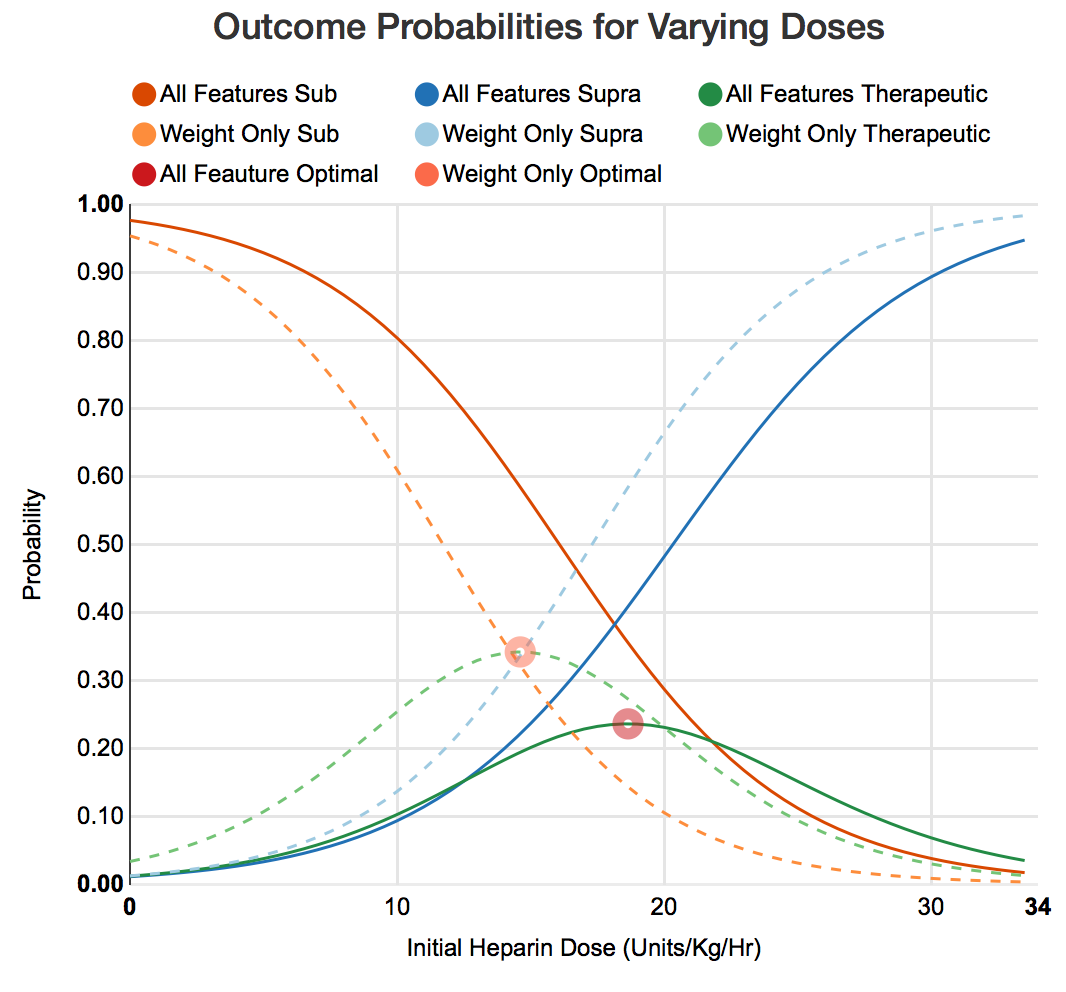
\includegraphics[width=0.7\textwidth]{source/figures/calc_graph.png}
\caption{\label{fig:calc_graph}Graph generated by the client software displaying an all features model vs. a weight-only model.}
\end{figure}

The frontend for the application was built in Angular.js. Angular.js is
client-side MVC (Model View Controller) framework that was chosen for
it's strengths in quick prototyping. The user interface was built on
Twitter Bootstrap, as it was familiar to the authors, is relatively easy
to use and offers built in responsive design. Additionally, it has many
CSS components such as nice forms and progress bars that are useful for
the design.\\
For graphing the D3.js, NV-D3 and Angular-nvd3 libraries were used which
enables inserting graphs using simple directives. Figure
\ref{fig:calc_graph} shows an example output of the standalone
calculator as seen in
\protect\hyperlink{appendix-2-application-user-interface}{Appendix 2} or
\href{https://hepstack-stage.herokuapp.com/\#/calc}{online}. The two
prominent dots represent the optimal doses for each model. Note that in
this example, the weight-only model predicts that the probability that
the patient will reach therapeutic state is higher than the all features
model.

\subsection{Backend}\label{backend}

\begin{figure}[H]
\noindent
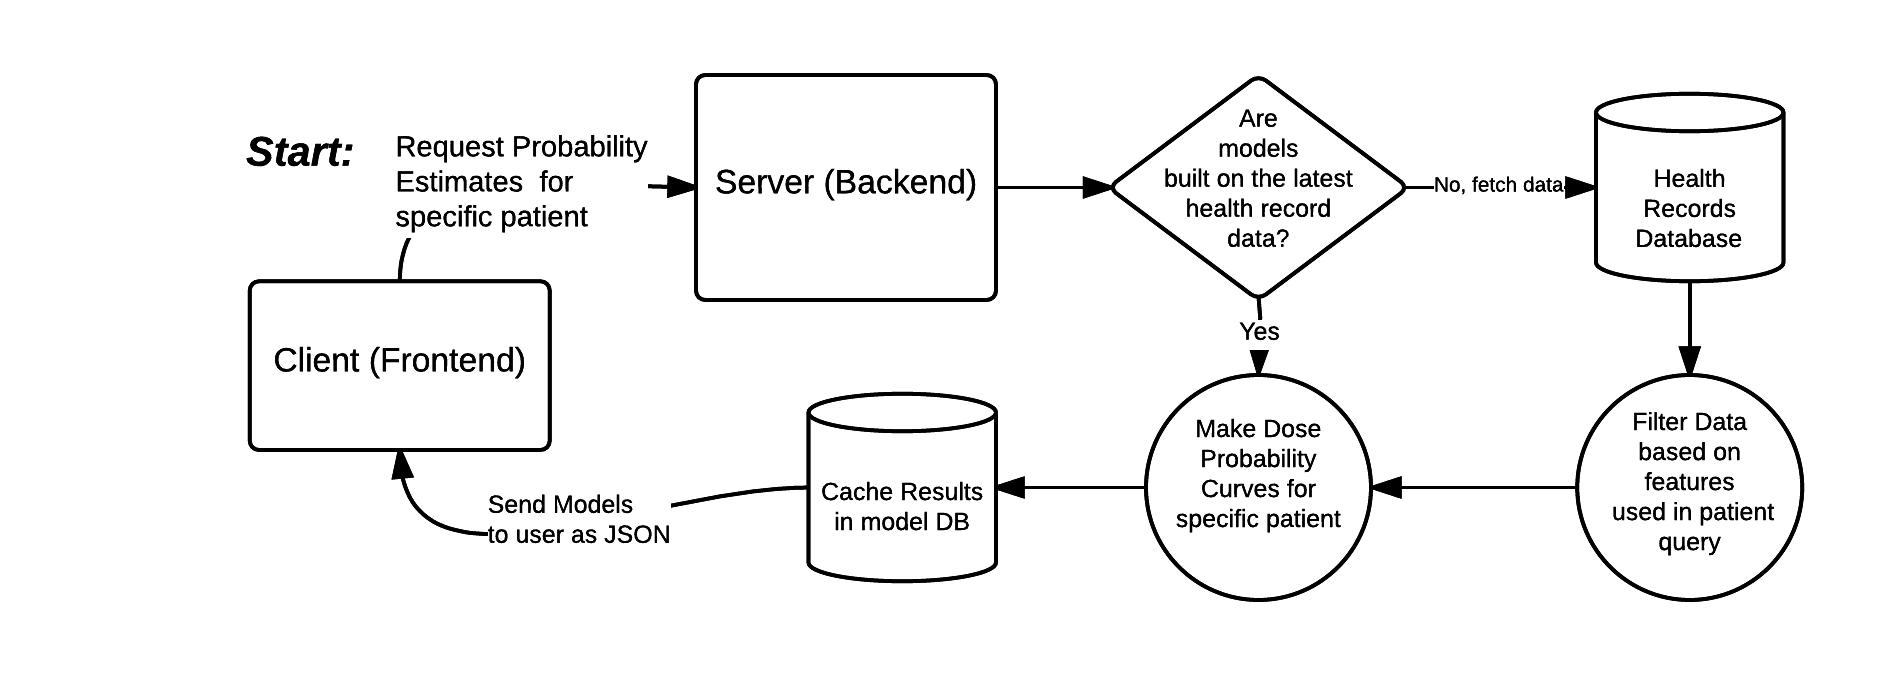
\includegraphics[width=1.05\textwidth]{source/figures/arch1.png}
\caption{\label{fig:flow1}Example of a typical client server interaction.}
\end{figure}

The backend for the application utilizes Python's Flask webframe work.
Data is stored in postgreSQL and accessed through the sqlalchemy object
relational mapping library. The frontend interfaces with the server via
a stateless RESTful API which enables the exchange of json data. Figure
\ref{fig:flow1} shows an example of how a client interacts with the
backend server currently.

\chapter{Heparin Survey}\label{heparin-survey}

\section{Survey Design}\label{survey-design}

\begin{figure}[H]
\centering
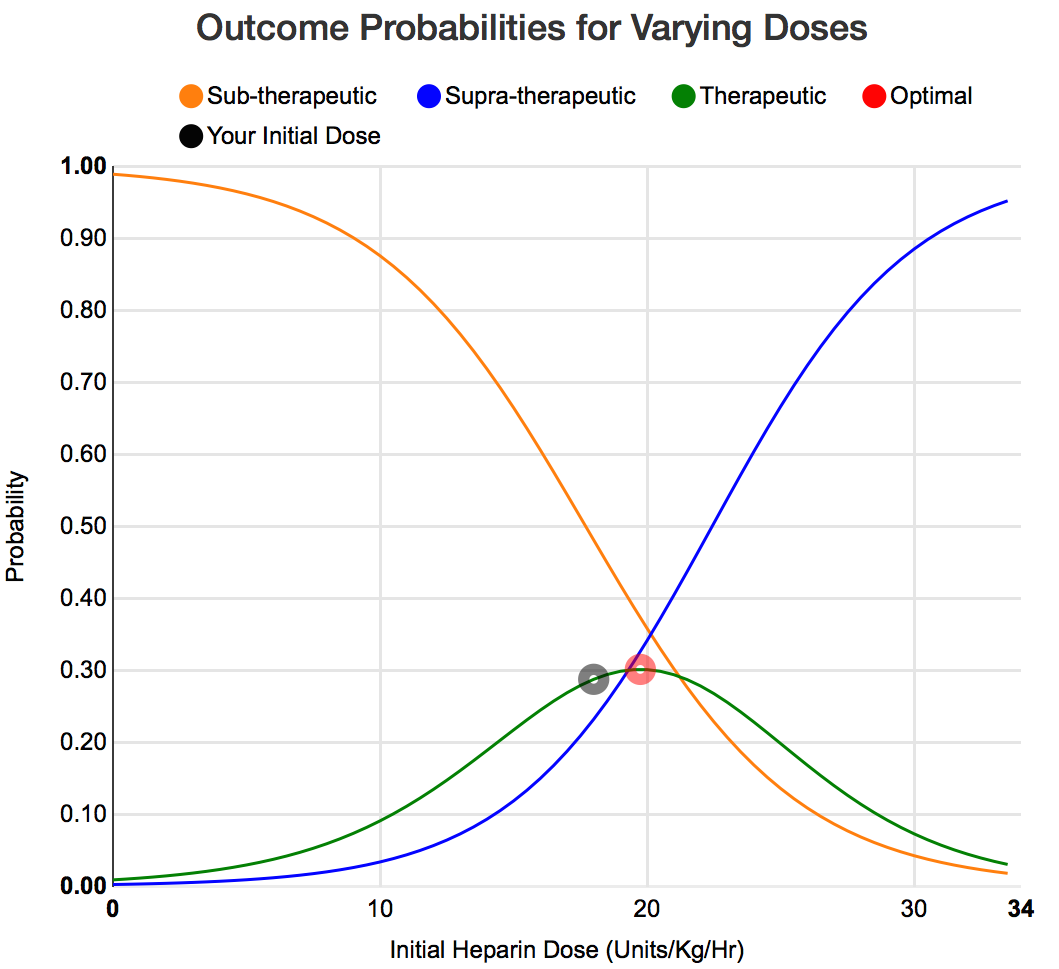
\includegraphics[width=0.7\textwidth]{source/figures/part3_iii.png}
\caption{\label{fig:part3_iii}Dosage curves with doctors initial dose plotted in black on the therapeutic curve.}
\end{figure}

The primary objective of the survey was to learn about the user
experience challenges involved with data-driven dosage techniques. To do
this a test interface was developed and several medical doctors of
varying disciplines attempted to use it. You can view the interface
\href{https://hepstack-stage.herokuapp.com/}{online} or in
\protect\hyperlink{appendix-2-application-user-interface}{Appendix 2}.
The survey consisted of five patient cases developed by domain experts
to cover multiple different use cases for heparin. A doctor would first
agree to a research disclosure, then fill out a short questionnaire
about their background and relevant experience (figure
\ref{fig:presurvey}). Next an instruction page was displayed explaining
the survey (figure \ref{fig:part3info1}, \ref{fig:part3info2}). Once the
doctor read over the instructions and guidelines, they were presented
with their first case which consists of some lab results and a short
admission note (figure \ref{fig:part3_i}). It was their task to
determine a potential infusion rate based on traditional heparin dosing
guidelines that were available to them. After choosing an infusion rate,
the optimal dose model was displayed (figure \ref{fig:part3_ii}). Unlike
the standalone calculator, the survey version of the graph does not
present the weight-only model. It does however plot the user's initial
infusion rate on the estimated therapeutic curve as a black dot, so they
can visualize the estimated dose versus their own dose (figure
\ref{fig:part3_iii}). The doctor then had the option of either adjusting
the dose or sticking with their initial dose. Whenever dosing the doctor
was able to leave notes to explain their reasoning. This task then was
repeated for the remaining four patients. After completing the test,
there was a short follow-up questionnaire consisting of a few questions
to gauge receptiveness to the tool and measure any change in confidence
when using the tool. Additionally, participants were asked for other
places they thought the tool could be used(figure \ref{fig:postsurvey}).
Due to financial and scope limitations, we could not compensate
participants for their time taking the survey. As a result all
volunteers were acquaintances or friend's of friends of the author.

\section{Architecture and
Implementation}\label{architecture-and-implementation}

The survey was implemented using the same technological stack as the
calculator (Angular.js and Bootstrap on the frontend, Python and Flask
on the backend). By utilizing a SPA (single page application)
methodology we were able to quickly iterate and make many revisions.
There were several candidate versions of the survey developed and tested
with domain experts for feedback. The final iteration allows for the
most direct input of comments from doctors, instead of relying on proxy
metrics such as time to complete cases that are similar too each other.

\chapter{Survey Results}\label{survey-results}

\section{Primary Findings}\label{primary-findings}

Participants adjusted their doses 72\% of time after reviewing the
model, which resulted in a higher probability of therapeutic outcome in
82\% of the adjustments. Additionally, participants reported greater
confidence when using the tool but also expressed some hesitation with
adopting the tool, often due to a lack of understanding of the
underlying models. More information follows. Access to the extended
survey results can be found in
\protect\hyperlink{appendix-1-full-survey-results}{Appendix 1}.

\section{Participant Profiles}\label{participant-profiles}

In total nine participants, all medical doctors completed the survey.
They range in experience from 4 to 32 years practicing. Of the nine, one
participant is a practicing physician in Ethiopia, and the rest practice
in the United States. One participant completed the study from a mobile
device and the others from a traditional laptop or desktop computer.
Five of the nine reported that they frequently prescribe heparin (at
least once a week) in their current position. One participant reported
prescribing it infrequently (once a month), two reported prescribing it
rarely and one reported prescribing never. All participants reported
that at sometime in the past they prescribed it frequently. The
participant medical specialties can be found in Table \ref{table:pre1},
but ranged from hematopathology to neuroendovascular surgery. Although
nine participants took the survey, one participant's infusion rates were
disqualified from the data analysis because they were 100 times greater
than the mean. Their comments were still kept for additional analysis.

\begin{table}[H]
\centering
\caption{Infusion rates before and after optimal dosage model was displayed. IR1 refers to the initial infusion rate, and IR2 refers the infusion rate chosen after viewing the model.}
\label{table:ir}
\begin{adjustbox}{max width=\textwidth}
\begin{tabulary}{15cm}{|L|RR|RR|RR|RR|RR|}
\hline
 & \multicolumn{2}{l|}{\textbf{Patient 1}} & \multicolumn{2}{l|}{\textbf{Patient 2}} & \multicolumn{2}{l|}{\textbf{Patient 3}} & \multicolumn{2}{l|}{\textbf{Patient 4}} & \multicolumn{2}{l|}{\textbf{Patient 5}} \\
\textbf{Suggested IR (Units/Kg/HR)} & \multicolumn{2}{l|}{19.7} & \multicolumn{2}{l|}{13.3} & \multicolumn{2}{l|}{15.9} & \multicolumn{2}{l|}{14.4} & \multicolumn{2}{l|}{17.5} \\ \hline
\textbf{Participant} & \textbf{IR 1} & \textbf{IR 2} & \textbf{IR 1} & \textbf{IR 2} & \textbf{IR 1} & \textbf{IR 2} & \textbf{IR 1} & \textbf{IR 2} & \textbf{IR 1} & \textbf{IR 2} \\ \hline
1 & 18 & 25 & 18 & 19 & 18 & 20 & 18 & 26 & 20 & 24 \\
2 & 18 & 19.8 & 18 & 13.9 & 13 & 16 & 12 & 14.7 & 13 & 17.6 \\
3 & 18 & 20.3 & 80 & 14.1 & 18 & 16.4 & 18 & 15 & 18 & 18 \\
4 & 12 & 12 & 15 & 15 & 12 & 15.9 & 15 & 15 & 12 & 17.3 \\
5 & 18 & 19.6 & 18 & 13.7 & 12 & 15.9 & 18 & 14.5 & 12 & 17.4 \\
6 & 18 & 18 & 18 & 18 & 13 & 13 & 12 & 14.8 & 0 & 0 \\
7 & 18 & 19.6 & 18 & 13.6 & 17 & 16 & 15 & 15 & 18 & 18 \\
8 & 18 & 19.7 & 18 & 13.8 & 13 & 16 & 12 & 14.7 & 18 & 18 \\ \hline
Min Dose & 12 & 12 & 15 & 13.6 & 12 & 13 & 12 & 14.5 & 0 & 0 \\
Max Dose & 18 & 25 & 80 & 19 & 18 & 20 & 18 & 26 & 20 & 24 \\
Standard Deviation & 2 & 4 & 22 & 2 & 3 & 2 & 3 & 4 & 6 & 7 \\
Mean Dose & 17 & 19 & 25 & 15 & 15 & 16 & 15 & 16 & 14 & 16 \\
Median Dose & 18 & 20 & 18 & 14 & 13 & 16 & 15 & 15 & 16 & 18 \\ \hline
\end{tabulary}
\end{adjustbox}
\end{table}

\section{Dose Differences}\label{dose-differences}

Each of the eight participants prescribed heparin twice to five
different patients, yielding a total of 80 infusion rates. In Table
\ref{table:ir}, for each patient there is a suggested optimal infusion
rate (IR) in the top header. This is the number that was displayed to
the user after they entered their initial infusion rate \emph{IR1}.
\emph{IR2} is the value they prescribed after viewing the optimal dosage
curve and the suggested infusion rate.\\
In the 40 trials, participants choose only 11 times to maintain their
initial infusion rate. In other words, 72\% of the time participants
adjusted their dose after viewing the model's suggested dose. In five of
the 29 times that a change was made, the change resulted in lower
probability of a therapeutic outcome than the original dose. All five of
these events occurred with participant number one, which may reflect the
user struggling to understand how to use the tool.

As for the reasoning for adjusting doses, they vary greatly as can be
seen in the appendix in Table \ref{table:YESNO}. Those who choose to
adjust towards the model values generally expressed trust in the model,
while some users, in particularly those who currently prescribe heparin
frequently where more wary of it. Some users explained they wanted to
adjust the infusion rate based on features that were not considered in
the model. Others expressed they wanted to adjust dosage using the
Anti-Xa Assay (an assay designed to monitor anticoagulant therapy (Reka
G Szigeti 2014).) Additionally, others expressed that their initial dose
was close enough, and that they preferred round numbers, since
administering doses in non-integer units is not always possible.

\section{User Feedback}\label{user-feedback}

Eight of the nine participants reported they felt more confident dosing
with the tool than without. One participant said it did not affect their
confidence. Although in general users reported greater confidence with
the tool, the majority expressed concern with adopting it due to a lack
of understanding of the models. As one participant noted the models are
``a bit of a `black box'.'' Other users noted that they were concerned
the tool was not adjusting for some specific complications. Another user
noted they were concerned about adopting it given there has not been a
validation trial for the technique. These concerns and others will be
addressed in the following section.

\chapter{Retrospective and Next
Steps}\label{retrospective-and-next-steps}

\section{User Concerns}\label{user-concerns}

Although most participants expressed that the dosing tool gave them
greater confidence, the majority also had reservations with adopting the
tool in their practice. Their common concern involved their
understanding of how the tool worked. This is concern appropriate, as it
reflects a conservative approach to experimenting on best practices in
patient care. One reason for their lack of understanding can be
attributed to the nature of this study, in that participants completed
the survey on their own time and were given no incentives for completing
the survey. As such, many users may have read the system explanation
quickly.\\
Additionally, the technique used for dosing, although not terribly
complex, is not trivial to understand. Physicians in general cannot be
asked to learn how a logistic regression works or how these models are
built. Simply speaking, their time is very valuable and limited. Thus,
experimental techniques need to be validated in formal clinical setting
with physicians who are invested in understanding and participating in a
trial of the new tools. Then once the techniques are validated others
can adopt them with greater confidence.\\
Another concern expressed was that the tool did not consider other
potential features when dosing patients. Although these features can be
added overtime, as the data becomes available and coded appropriately,
this concern speaks to the greater issue of user interaction with the
model. In its current state the standalone calculator allows physicians
to view the weight-only model and the all features model. This gives
them a better understanding of how these features change the therapeutic
curve. Future versions of this tool should allow the user to enable and
disable a given feature, so they can have a better understanding of the
effects of the feature on the model outcome. This understanding could
potentially come in the form of additional visualizations like the
original graph or arguably better in the form of written descriptions,
e.g. ``The SOFA score causes a deviation of 3\% from normal dosing.''
The initial version of this project included a crude nearest neighbor
visualization, but that feature was not incorporated in the final
version due to time limitations. Increasing user interaction with the
tool will hopefully address some knowledge and trust issues with the
current system.

\section{Shortcomings in the Survey}\label{shortcomings-in-the-survey}

This study has no shortage of problems. The problems generally come from
a lack of resources, in terms of time and money. A funded study would
allow for a greater number of participants with specific ICU expertise.
Additionally the participant selection process would not be limited to
friends of the researchers, which may have skewed the results. Funding
would also allow for time for researchers to work with participants to
better understand the model. Given the problems with the survey, and
limited number of participants, the results are still very valuable as
they clearly reveal areas for future improvement in the system.

\section{Future Implementations}\label{future-implementations}

The experimental nature of this project has lead to a software
implementation that is limited in several ways. The codebase served its
purpose as a tool for a research study fairly well, but it is not ``real
world'' ready in its current form. In future versions we'd like to see
improved logging, system documentation, automated unit testing on
builds, and better scaling performance (possibly utilizing redis).
Additionally, the overall design should be more modular, such that it is
easier to try out and compare different candidate models (e.g.~Ensemble
Learning, Neural Networks, SVMs, etc.) on different drugs. Automated
testing could even run trial comparisons and compute statistics on
models. From a data processing perspective, an entire subsystem should
be designed and built for selecting data from the medical records
database and translating it into a suitable form for models. There
should also be tools for validating the cohort selection. This is not a
trivial task when working with a specific medical record database, and
becomes much more challenging when attempting to interface with other
databases. Defining the generic interface used for selecting the cohort
from the database will be challenging. Finally the data will also need
to be validated and then translated (coded) to appropriate values for a
given model.\\
On the frontend, user analytics could be improved, as it would be ideal
to know more about the user's device and how they interact on a
per-click basis. One final improvement on the client would be modifying
the data model, such that instead of requesting an estimate for a
specific patient, the client requests a static model that has been
precomputed on the server using the latest dataset. Then the user can
manually modify features and the estimated probability curves are
computed client side. This should allow for a much more responsive
experience for the user, providing them instantaneous feedback for each
feature change made, instead requiring a request to the server for each
change. The dosage curves could be computed in a separate thread using
web workers. Additionally, by implementing the predictions client side,
patient data does not need to be transfered to an external server
(easing HIPAA compliance), and the client can be fully functional
offline which is ideal for low resource environments such as developing
countries.

\chapter{Conclusion}\label{conclusion}

The central focus of this study was to implement an interactive
data-driven dosage tool and test its usability with medical doctors.
While doing this we learned about domain specific, technical, and
usability challenges. The goal of our work was to provide sufficient
information such that a new version could be built and tested in a
formal clinical setting. While the majority of participants felt more
confident prescribing heparin using the tool, they also overwhelming
expressed a need for a greater understanding of the underlying models
making the predictions. This speaks to a usability problem that will be
addressed in future versions by creating a more interactive, learning
based tool. The future architecture presented will also open the door to
dosing other drugs and trying out other models beyond logistic
regression. These techniques will provide personalized insight in
complex cases involving unique patient cohorts. Without question, in
time the computer's roll in prescribing drugs will grow, leading to
improved quality of care for patients while decreasing hospital stay
times and the cost of care.

\newpage

\hypertarget{appendix-1-full-survey-results}{\chapter*{Appendix 1: Full
Survey Results}\label{appendix-1-full-survey-results}}
\addcontentsline{toc}{chapter}{Appendix 1: Full Survey Results}

\begin{itemize}
\tightlist
\item
  Project Resources

  \begin{itemize}
  \tightlist
  \item
    \href{https://github.com/joer14/ThesisPaper/blob/master/publicCodeEn.zip?raw=true}{Link
    to Client Side and Server Side Code Archive (Password Protected)}
  \item
    \href{https://hepstack-stage.herokuapp.com/responses}{Link to Raw
    Survey Results Data}
  \end{itemize}
\end{itemize}

\section{Presurvey Questionnaire:}\label{presurvey-questionnaire}

\begin{enumerate}
\def\labelenumi{\arabic{enumi}.}
\tightlist
\item
  What are your credentials? - MD - MD/PhD - NP - Other\\
\item
  What is primary medical specialty? - (e.g.~Obstetrics)\\
\item
  How long have you been practicing in a clinical setting? - (e.g.~10
  years)\\
\item
  In your current position how often do you prescribe heparin or other
  anticoagulants?

  \begin{itemize}
  \tightlist
  \item
    Frequently - (at least once a week)
  \item
    Infrequently - (once a month)
  \item
    Rarely - (once a year or so)
  \item
    Never
  \end{itemize}
\item
  In the past did you ever prescribe heparin or other anticoagulants
  more frequently? If so, how often?

  \begin{itemize}
  \tightlist
  \item
    Frequently - (at least once a week)\\
  \item
    Infrequently - (once a month)
  \item
    Rarely - (once a year or so)
  \item
    Never - I haven't prescribed heparin or other anticoagulants
  \end{itemize}
\item
  Have you ever worked in an ICU? If so, to what extent?

  \begin{itemize}
  \tightlist
  \item
    (e.g During my residency I had 2 rotations lasting roughly 10 weeks
    each in different ICUs.)
  \end{itemize}
\end{enumerate}

\begin{table}[H]
\centering
\caption{Presurvey Results Questions 1-5}
\label{table:pre1}
\begin{adjustbox}{max width=\textwidth}
\begin{tabulary}{1.5\textwidth}{|L|LLLLL|}
\hline
Participant & Credential & Specialty & Years Practicing & Current Heparin Experience & Past Heparin Experience \\ \hline
1 & MD & Pediatric Hematology & 30 & Infrequently & Frequently \\
2 & MD & Hematopathology & 32 & Never & Frequently \\
3 & MD & Neuroradiology & 30 & Rarely & Frequently \\
4 & MD & neurosurgery, neurocritical care, clinical informatics & 16 & Frequently & Frequently \\
5 & MD & Neurology & 15 & Frequently & Frequently \\
6 & MD & Pediatric Critical Care & 28 & Frequently & Frequently \\
7 & MD & Neurology & 4 & Frequently & Frequently \\
8 & MD & Neuroendovascular Surgery & 12 & Frequently & Frequently \\ \hline
\end{tabulary}
\end{adjustbox}
\end{table}

\begin{table}[H]
\centering
\begin{adjustbox}{max width=\textwidth}
\caption{Presurvey Results Question 6}
\label{table:pre2}
\begin{tabularx}{\textwidth}{|l|X|}
\hline
Participant & ICU Experience \\ \hline
1 & I have served as a consultant in the PICU for 30 years \\ \hline
2 & Surgery internship: vascular surgery patients - 2 mos \\ \hline
3 & About 10 months of ICU during training - mixture of medical, surgical, and cardiac \\ \hline
4 & In residency training x 7 years and as faculty x 9.5 years \\ \hline
5 & Approximately 1 to 5 patients per month in ICU. \\ \hline
6 & Residency (3 month long rotations), Fellowship (3 years), Attending (13 years) \\ \hline
7 & I have bimonthly rotations there \\
8 & No \\ \hline
\end{tabularx}
\end{adjustbox}
\end{table}

\section{Follow Up Survey}\label{follow-up-survey}

\begin{enumerate}
\def\labelenumi{\arabic{enumi}.}
\tightlist
\item
  Did you feel more confident prescribing heparin when using the models?

  \begin{itemize}
  \tightlist
  \item
    I felt more confident using the models.\\
  \item
    I felt less confident using the models.
  \item
    The models did not affect my confidence.
  \end{itemize}
\item
  What hesitations do you have about adopting statistical dosing
  tools?\\
\item
  Are there any specific areas you'd like to see a tool like this being
  used?\\
\item
  If you have any further comments, questions, suggestions, ideas for
  improvement, etc please enter them below.
\end{enumerate}

\begin{table}[H]
\centering
\caption{Follow Up Survey Responses Question 1 and Question 2}
\label{my-label}
\begin{tabularx}{\textwidth}{|l|l|X|}
\hline
 & Q1 & Question 2 - Hesitations \\ \hline
1 & More & need a bit more data about renal function and overall status \\ \hline
2 & More & You are stepping out of the realm of current standard practice. You are relying on 1) the data used in the model reflecting the patient group seen in your practice, 2) the statistical methods used being the most appropriate. \\ \hline
3 & More & A bit of a 'black box' - I would want to see more about validation before fully implementing \\ \hline
4 & Equally & would like to know more about the stats and the mechanisms that are responsible for the predictions \\ \hline
5 & More & Lack of prospective trial using this method to provide validation of this tool \\ \hline
6 & More & Still have to take in consideration other complications with regard to thrombus formation, bleeding risk, clearance (renal injury), other coagulation factors, etc. \\ \hline
7 & More & The fractions in calculation makes hard to adminster we could round up for example 18.2 to 18 that way it would be more applicable \\ \hline
8 & More & None \\ \hline
9 & More & None; very helpful \\ \hline
\end{tabularx}
\end{table}

\begin{table}[H]
\centering
\caption{Follow up  Survey Responses Question 3}
\label{my-label}
\begin{tabularx}{\textwidth}{|l|X|}
\hline
Participant & Question 3 - Other Areas \\ \hline
1 & yes - in the ICU \\ \hline
2 & Potentially this could be a great tool for patients on multiple drugs simultaneously - are there models that will help predict more accurately what type of dose adjustments should be made for patients on multiple heart failure meds e.g. \\ \hline
3 & Other pharmaceuticals, e.g. antibiotics requiring levels (Vancomycin, Gentamycin, etc) \\ \hline
4 & medical care of patients in general particularly for blood sugar, pain control \& sedation, etc. \\ \hline
5 & Warfarin dosing? \\ \hline
6 & I think it would be helpful in the ICU as a guide. \\ \hline
7 & Yes. Specially in fluid management in shock patients \\ \hline
8 & protocolizeed approaches. \\ \hline
9 & Treatment for PE, acute extremity thrombosis, stroke \\ \hline
\end{tabularx}
\end{table}

\begin{table}[H]
\centering
\caption{Follow up  Survey Responses Question 4}
\label{my-label}
\begin{tabularx}{\textwidth}{|l|X|}
\hline
Participant & Question 4 - Other Comments \\ \hline
2 & It would be interesting to know if the dosing model works the same, or similarly among different patient groups (race, sex, BMI etc) and if not are there ways to adapt for these factors.,The dosing tool model is an excellent idea. \\ \hline
8 & Create your own web page where people can go and use....similar to Angiocalc.com \\ \hline
9 & Would be good to get one more feedback calculation after adjusted the dose for a confirmation since I made mistakes by a factor of 10 \\ \hline
\end{tabularx}
\end{table}

\begin{table}[H]
\centering
\caption{Timing Results, Where T1 is amount of time in seconds between displaying the case and the doctors first dose is prescribed and where T2 is amount of time in seconds that the doctor viewed the model before submitting their second dose.}
\label{table:timing}
\begin{adjustbox}{max width=\textwidth}

\begin{tabulary}{15cm}{|L|LL|LL|LL|LL|LL|r|}
\hline
 & \multicolumn{2}{l|}{Patient 1} & \multicolumn{2}{l|}{Patient 2} & \multicolumn{2}{l|}{Patient 3} & \multicolumn{2}{l|}{Patient 4} & \multicolumn{2}{l|}{Patient 5} & \multicolumn{1}{l|}{} \\ \hline
\textbf{Participant} & \textbf{T1} & \textbf{T2} & \textbf{T1} & \textbf{T2} & \textbf{T1} & \textbf{T2} & \textbf{T1} & \textbf{T2} & \textbf{T1} & \textbf{T2} & \multicolumn{1}{l|}{\textbf{Total Time}} \\ \hline
1 & 67 & 38 & 21 & 29 & 30 & 37 & 38 & 27 & 23 & 44 & 5 mins, 54 secs \\
2 & 136 & 42 & 49 & 45 & 53 & 33 & 98 & 26 & 112 & 19 & 10 mins, 13 secs \\
3 & 38 & 38 & 32 & 34 & 52 & 34 & 68 & 238 & 45 & 28 & 10 mins, 7 secs \\
4 & 23 & 69 & 50 & 53 & 237 & 79 & 96 & 32 & 86 & 72 & 13 mins, 17 secs \\
5 & 11 & 8 & 87 & 15 & 24 & 25 & 9 & 18 & 54 & 7 & 4 mins, 18 secs \\
6 & 55 & 60 & 25 & 84 & 38 & 21 & 85 & 46 & 51 & 22 & 8 mins, 7 secs \\
7 & 70 & 86 & 45 & 58 & 442 & 51 & 95 & 36 & 94 & 36 & 16 mins, 53 secs \\
8 & 135 & 83 & 54 & 40 & 29 & 19 & 29 & 18 & 44 & 50 & 8 mins, 21 secs \\ \hline
\textbf{Min Time} & 11 & 8 & 21 & 15 & 24 & 19 & 9 & 18 & 23 & 7 & \multicolumn{1}{l|}{} \\
\textbf{Max Time} & 136 & 86 & 87 & 84 & 442 & 79 & 98 & 238 & 112 & 72 & \multicolumn{1}{l|}{} \\
\textbf{Standard Deviation} & 47 & 26 & 21 & 21 & 150 & 20 & 35 & 74 & 30 & 20 & \multicolumn{1}{l|}{} \\
\textbf{Mean Time} & 67 & 53 & 45 & 45 & 113 & 37 & 65 & 55 & 64 & 35 & \multicolumn{1}{l|}{9 mins, 39 secs} \\
\textbf{Median Time} & 61 & 51 & 47 & 42.5 & 45 & 33.5 & 76.5 & 29.5 & 52.5 & 32 & \multicolumn{1}{l|}{7 mins, 51 secs} \\ \hline
\end{tabulary}
\end{adjustbox}
\end{table}

\begin{table}[H]
\centering
\caption{Bolus Information}
\label{my-label}
\begin{tabular}{|l|lllll|}
\hline
Participant & Patient 1 & Patient 2 & Patient 3 & Patient 4 & Patient 5 \\ \hline
1 & 80 & 80 & 60 & 80 & 60 \\
2 & 80 & 60 & 0 & 40 & 0 \\
3 & 5000 & 5000 & 80 & 80 & 80 \\
4 & 5000 & 6000 & 3500 & 6000 & 5400 \\
5 & 80 & 80 & 0 & 80 & 0 \\
6 & 80 & 80 & 0 & 44.5 & 0 \\
7 & 80 & 80 & 0 & 60 & 80 \\
8 & 80 & 80 & 0 & 60 & 80 \\ \hline
\end{tabular}
\end{table}

\begin{table}[H]
\centering
\caption{Reasons participants choose to adjust or not to adjust their initial dose.}
\label{table:YESNO}
\begin{adjustbox}{max width=1\textwidth}
\begin{tabulary}{1.2\textwidth}{|l|l|l|L|}
\hline
Participant & Patient \# & Adjust or Not & Why \\ \hline
1 & 1 & Yes & need to get her there \\
  & 2 & Yes & to get him there \\
  & 3 & Yes & same reason as before - under dosed her \\
  & 4 & Yes & need to get there \\
  & 5 & Yes & to prevent further thrombosis \\ \hline
2 & 1 & Yes & I'm relying on the model \\
  & 2 & Yes & Model is probably better than my prediction as pt is pretty heavy \\
  & 3 & Yes & model \\
  & 4 & Yes & Bolus dose may well be too small \\
  & 5 & Yes & I am relying on this model \\ \hline
3 & 1 & Yes & model is close to my prediction and based on real data \\
  & 2 & Yes & I actually made a mistake in my initial calculation! \\
  & 3 & Yes & Makes sense, older pt may need less as indicated by model \\
  & 4 & Yes & Graphs indicate higher likelihood of therapeutic result for this patient profile, and it seems reasonable to my initital estimate \\
  & 5 & No & Close enough - no compelling reason to change \\ \hline
4 & 1 & No & No PE yet.  Would follow labs to see where she goes. \\
  & 2 & No & has active PE.  will adjust infusion based on individual response for Xa level. \\
  & 3 & Yes & No clear emergency on type of dosing.  Pt stroke is completed.  Likely will not need a decompression unless bleeding occurs post heparinization. \\
  & 4 & No & it's about the same and I'd rather be slightly high than low. \\
  & 5 & Yes & if this is more likely to get to a therapeutic window quickly, would choose to do so. \\ \hline
6 & 1 & No & Creatinine was elevated \\
  & 3 & No & Risk of intracranial bleed \\
  & 4 & Yes & Risk of continued thrombus greater than risk of bleeding \\
  & 5 & No & Lack of evidence in this condition. \\ \hline
7 & 4 & No & It is fairly equal. No meed to calculate the fractions \\
  & 5 & No & Again only fractions \\ \hline
8 & 1 & Yes & model said would be better. \\
  & 2 & Yes & per model. \\
  & 3 & Yes & per model. \\
  & 4 & Yes & per model. \\ \hline
9 & 1 & Yes & recommended \\
9 & 2 & Yes & recommended \\ \hline
\end{tabulary}
\end{adjustbox}
\end{table}

\newpage

\hypertarget{appendix-2-application-user-interface}{\chapter*{Appendix
2: Application User
Interface}\label{appendix-2-application-user-interface}}
\addcontentsline{toc}{chapter}{Appendix 2: Application User Interface}

Below are screenshots of the calculator application and survey
application in use. You encouraged to try them out yourself directly at
\url{https://hepstack-stage.herokuapp.com/}.

\section{Calculator Interface}\label{calculator-interface}

\begin{figure}[H]
\noindent
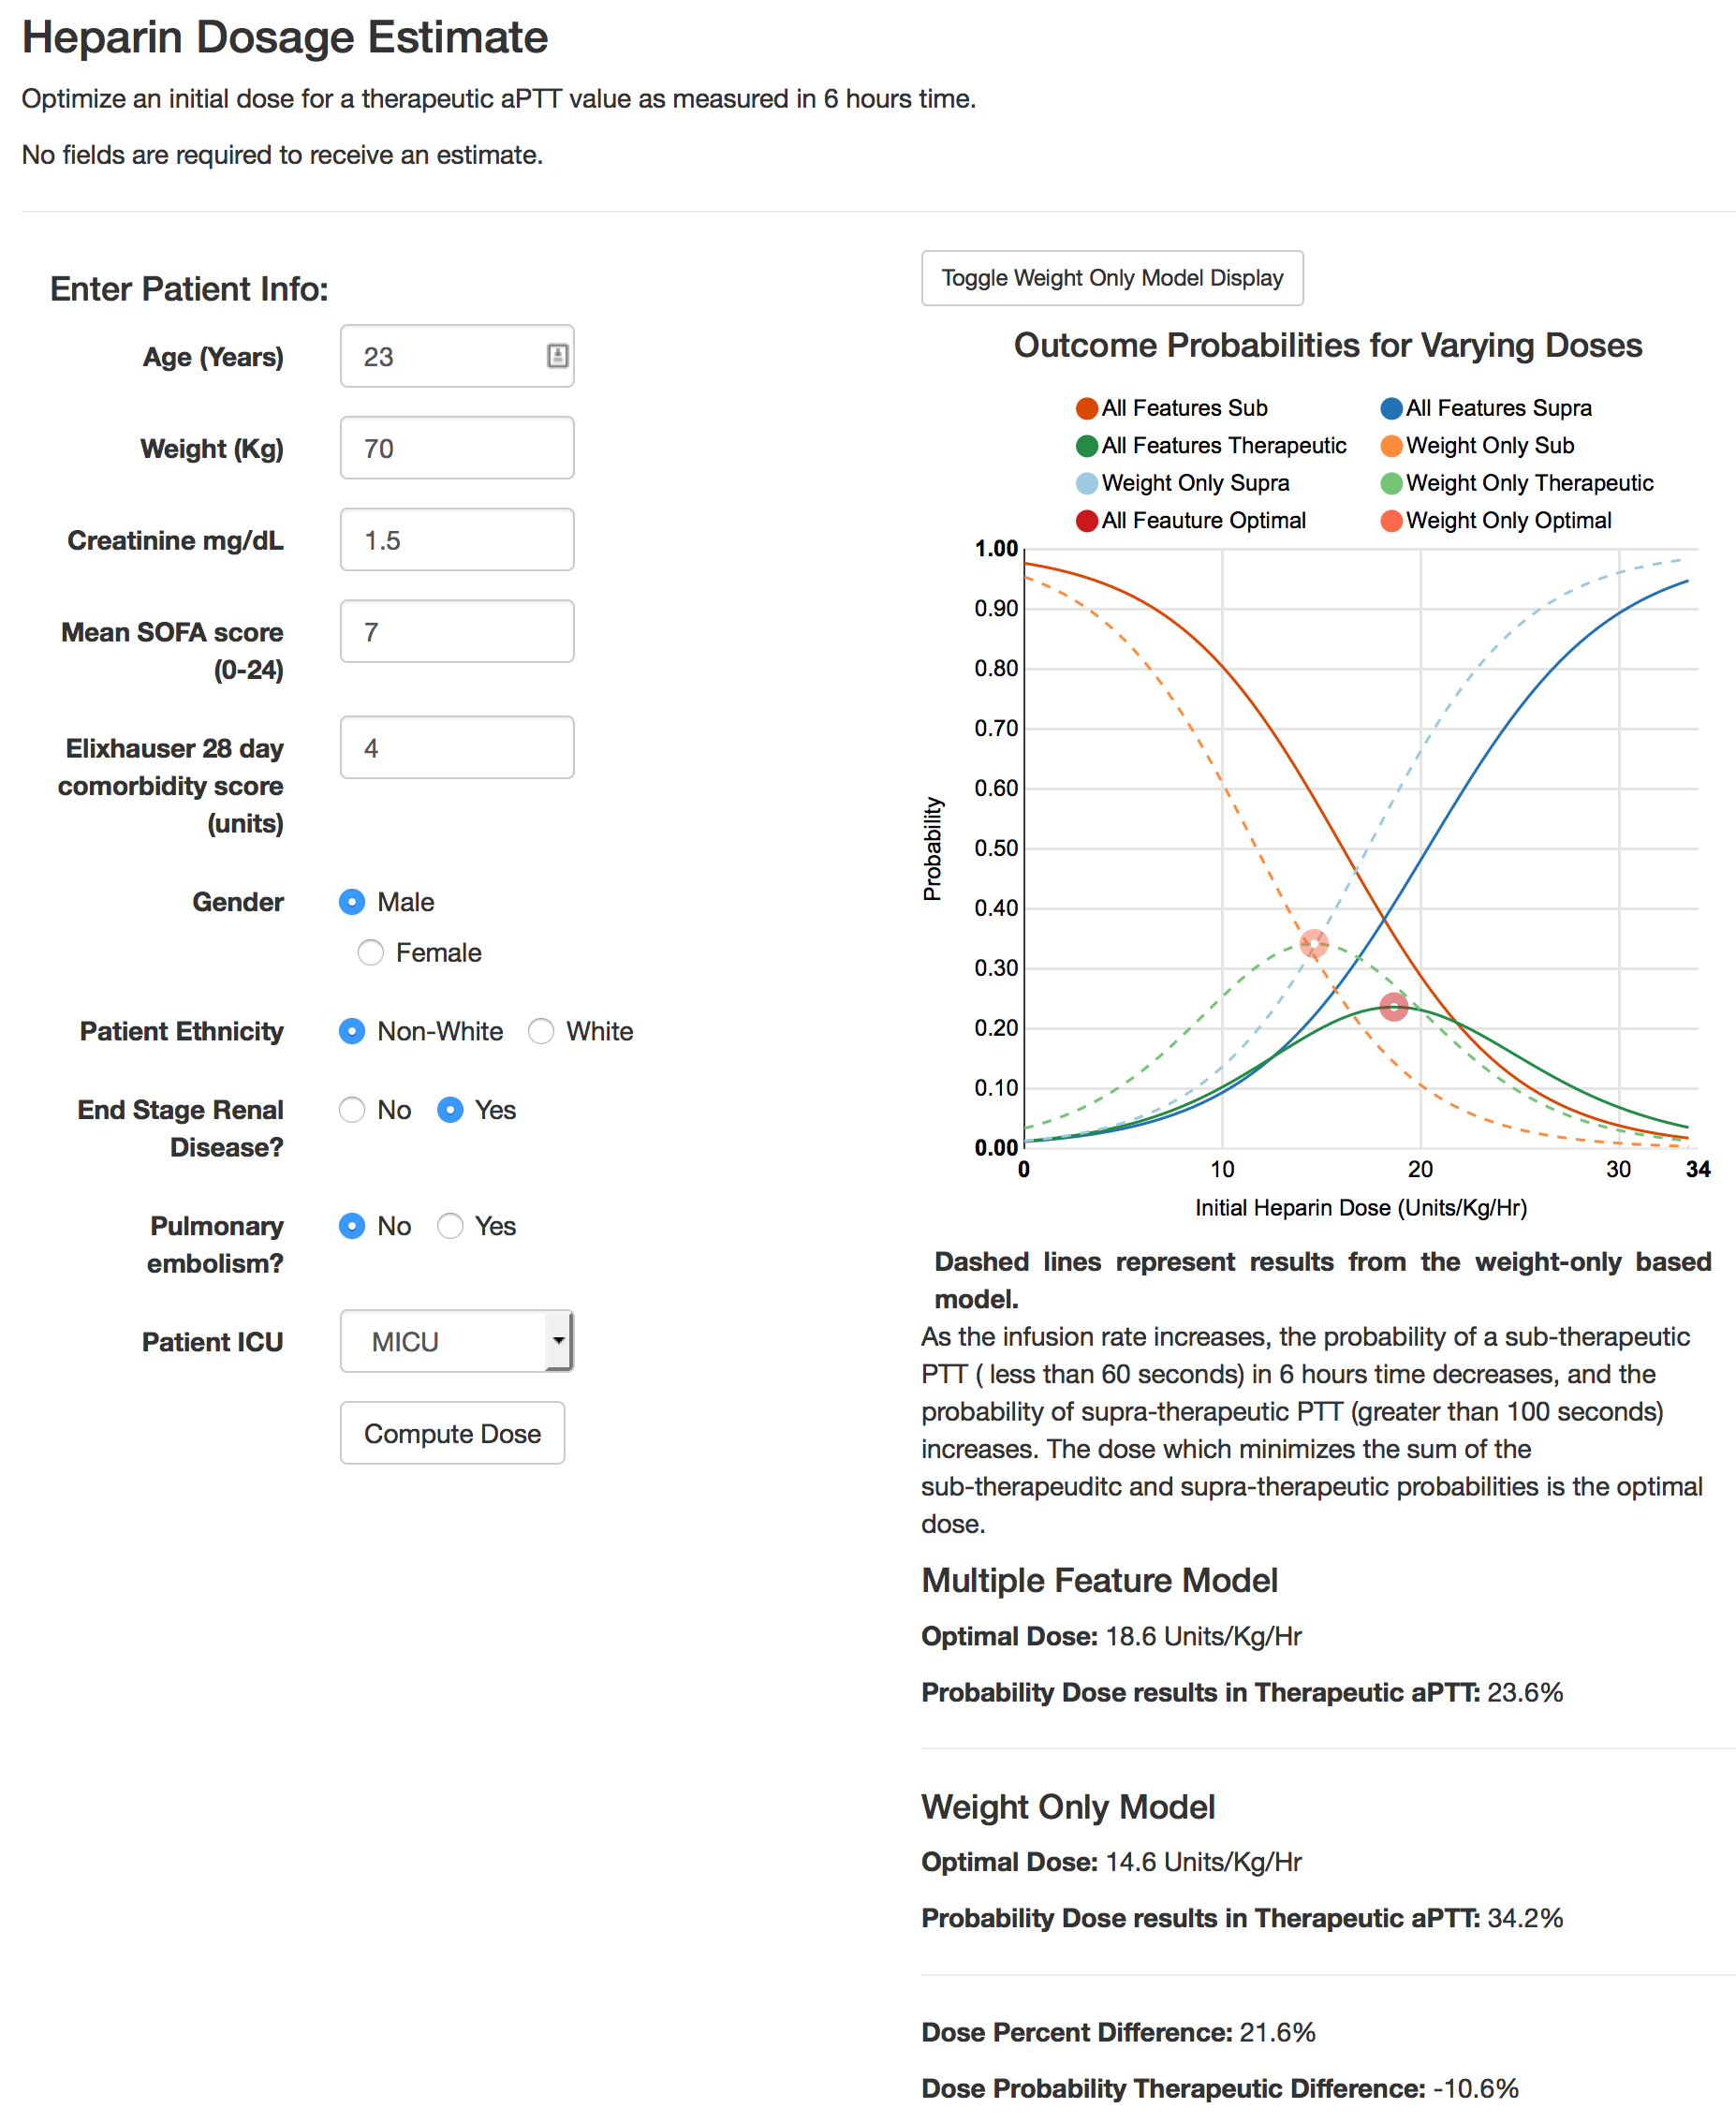
\includegraphics[width=1\textwidth]{source/figures/calc_full.png}
\caption{\label{fig:calc_full}The standalone calculator user interface with patient data entered.}
\end{figure}

\section{Survey Interface}\label{survey-interface}

\begin{figure}[H]
\noindent
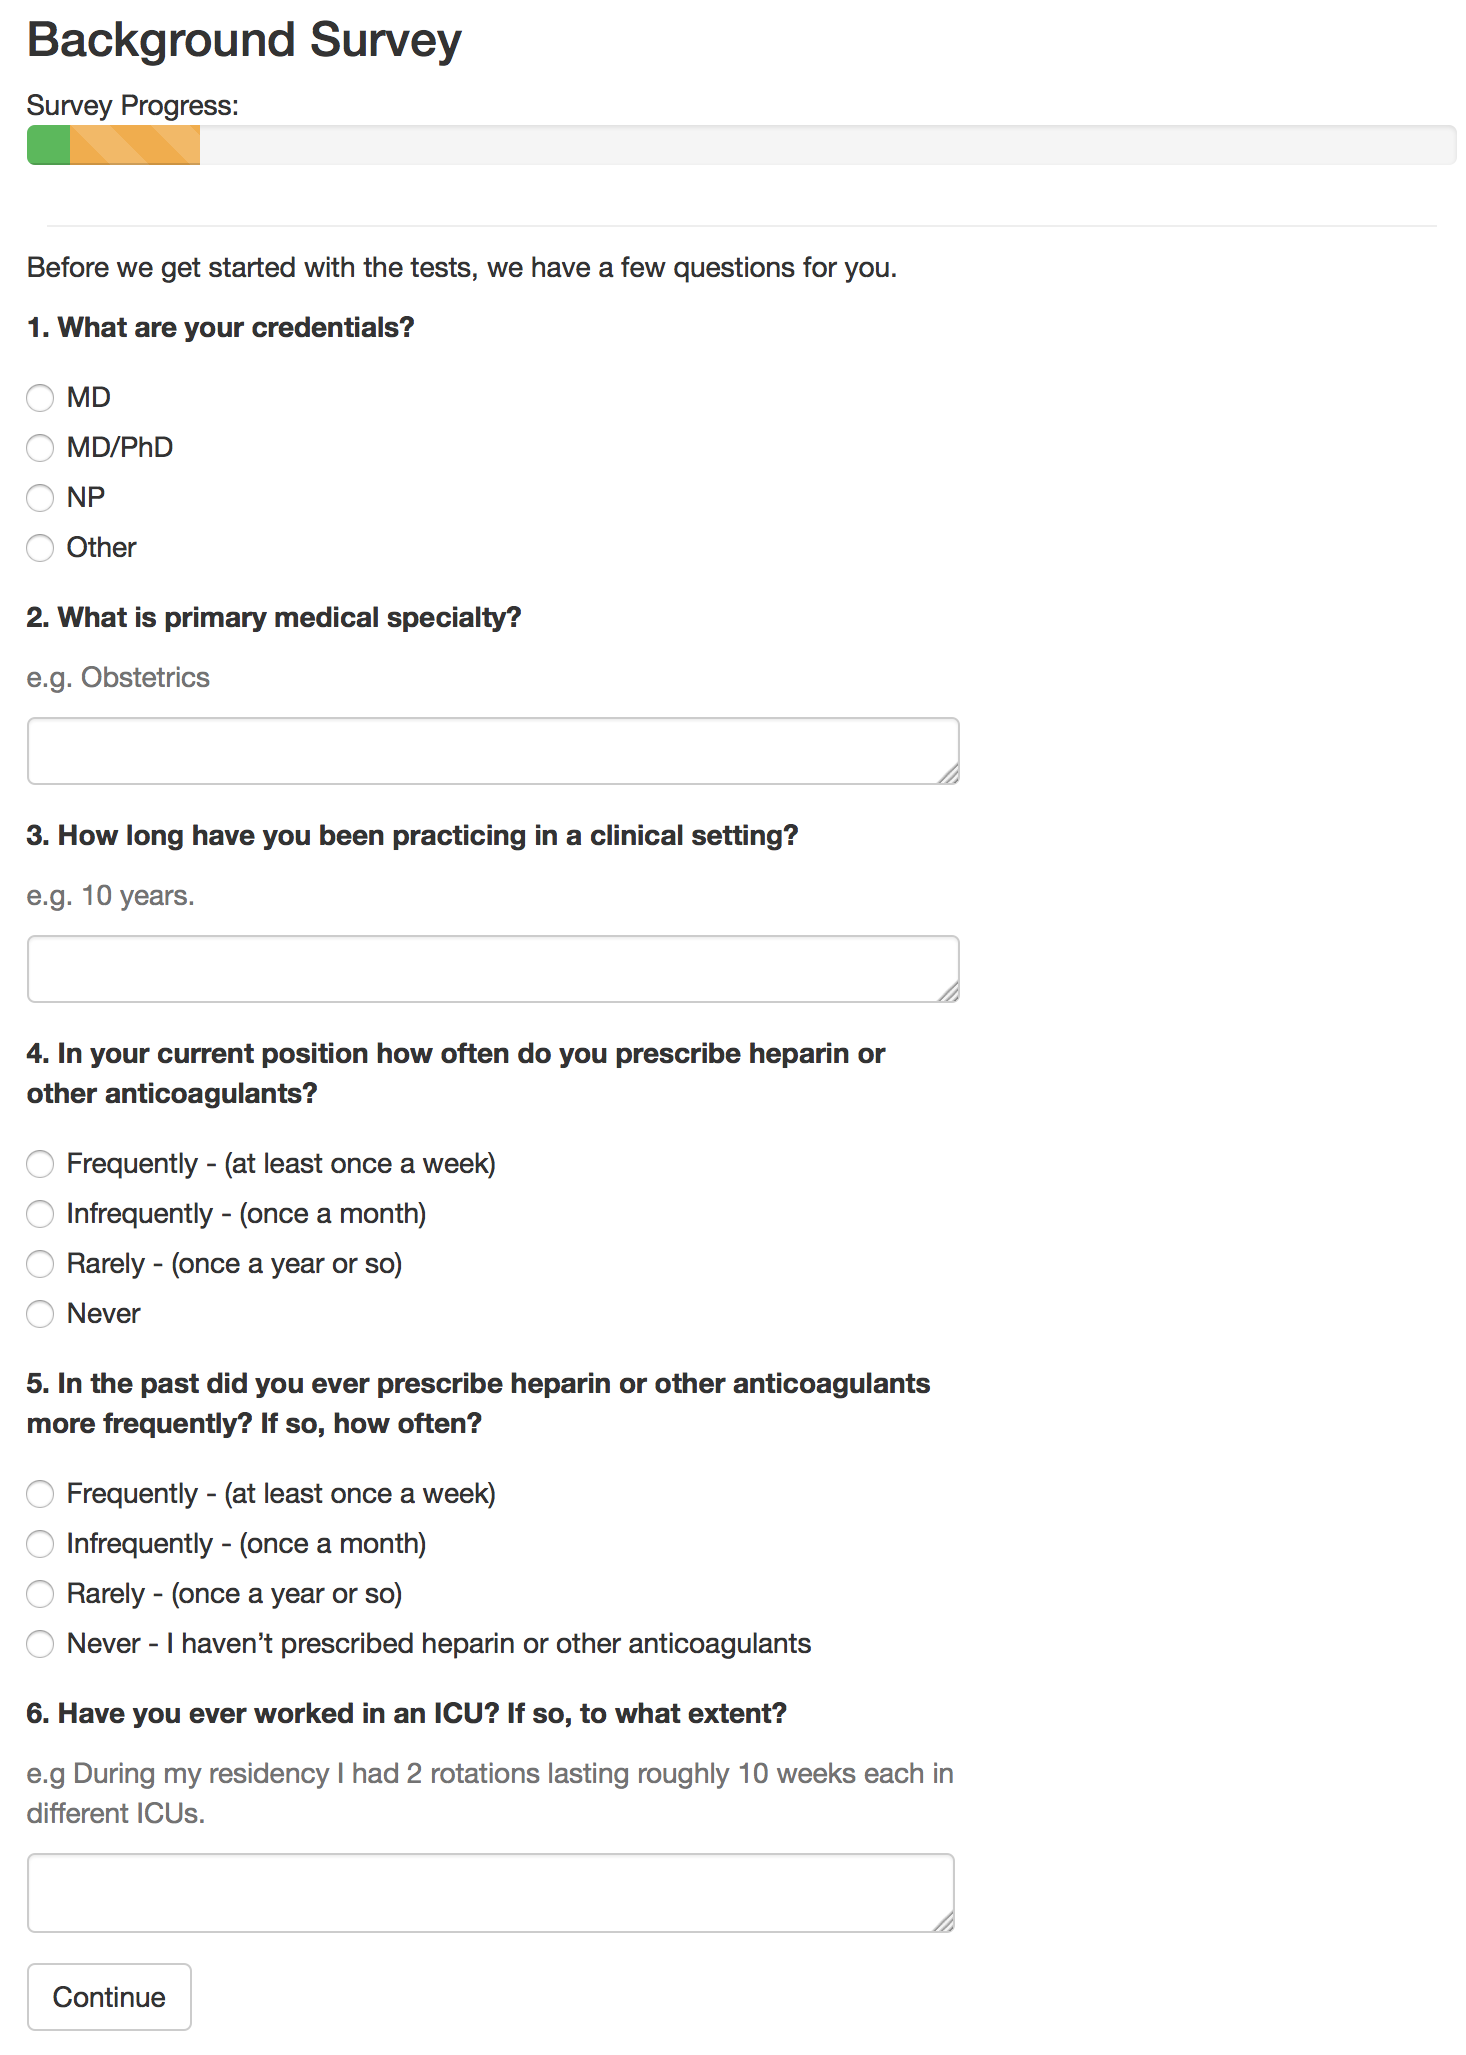
\includegraphics[width=1\textwidth]{source/figures/presurvey2.png}
\caption{\label{fig:presurvey}The questionnaire presented to study participants before they are able to  dose patients.}
\end{figure}

\begin{figure}[H]
\noindent
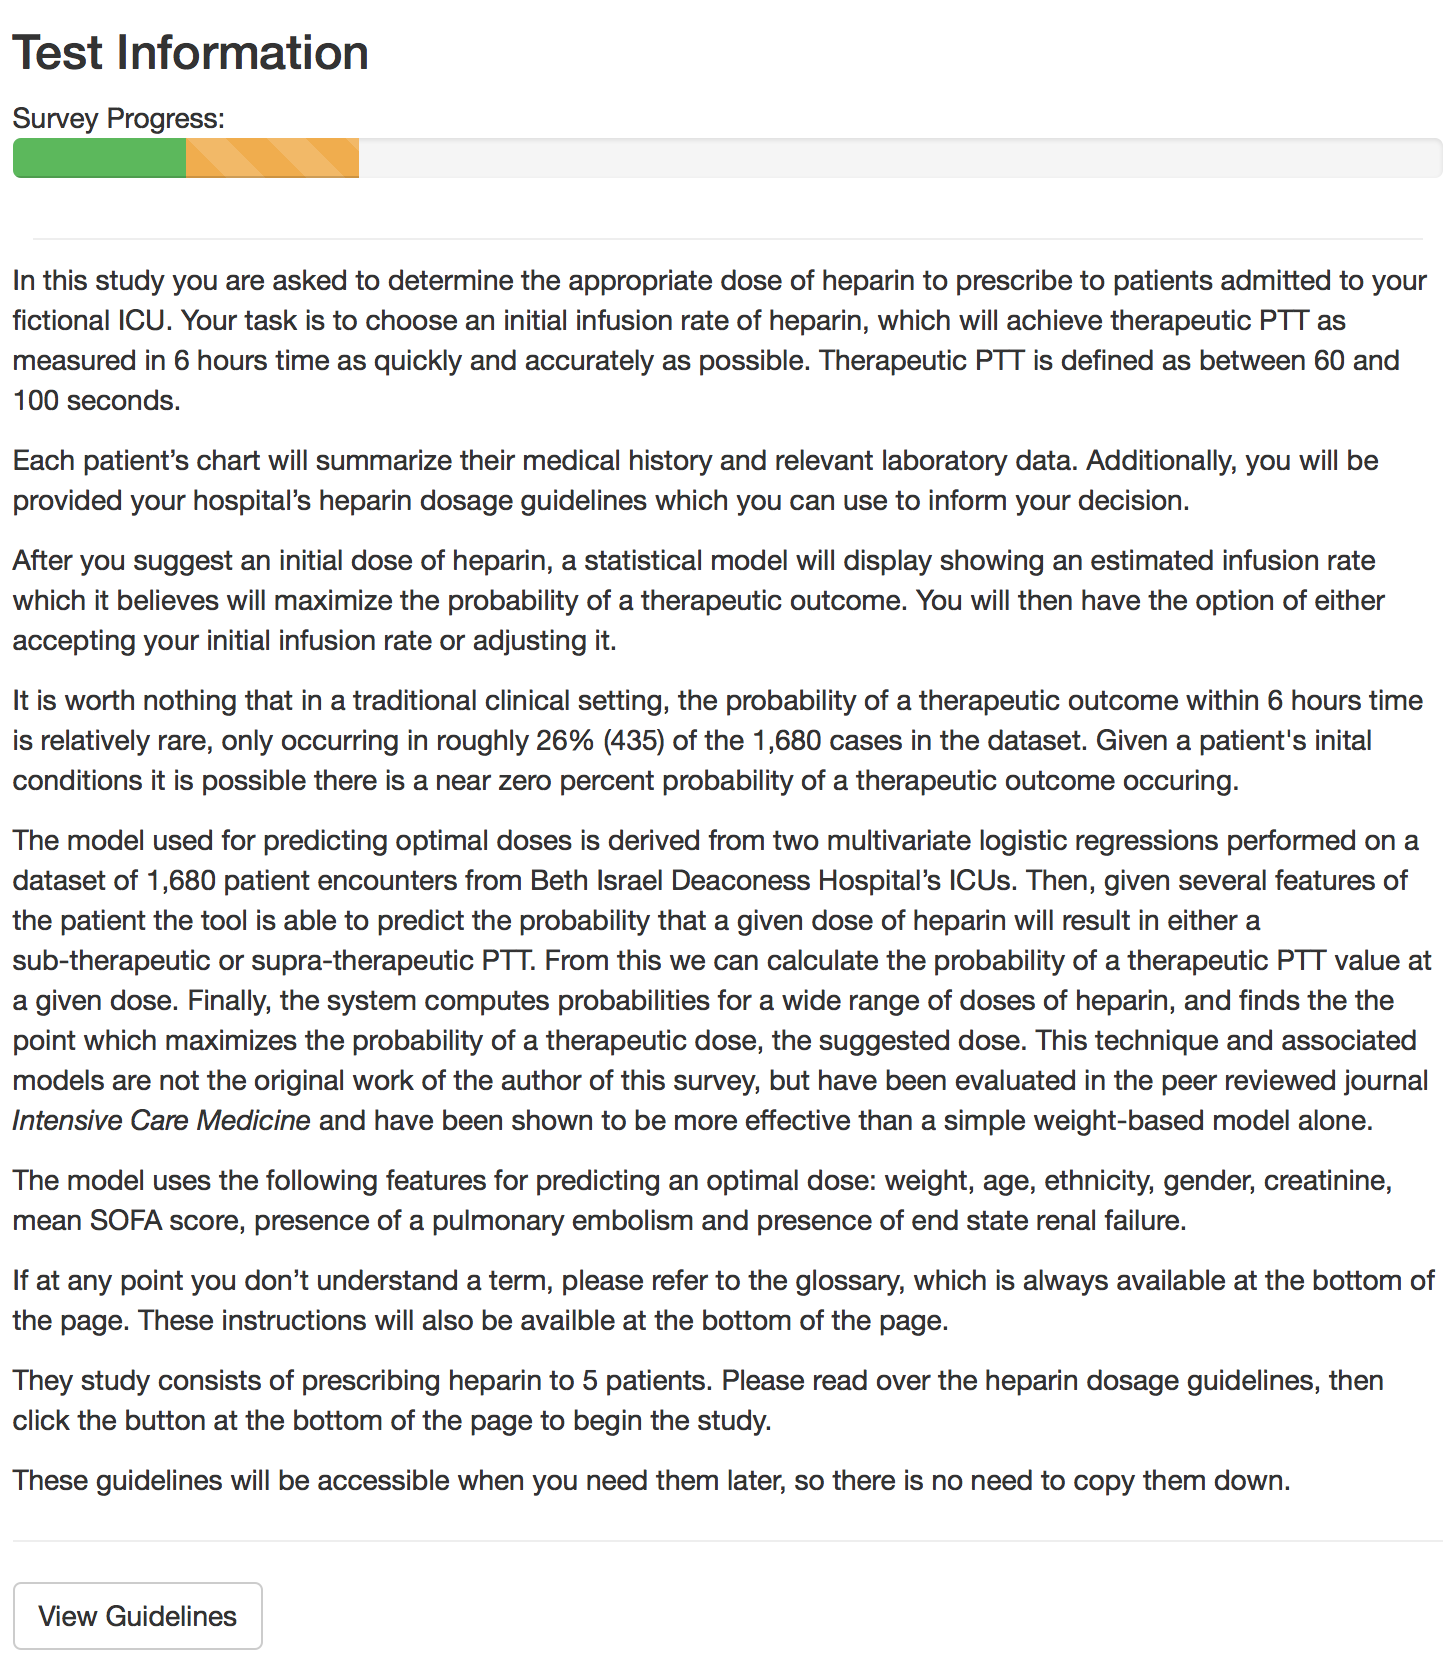
\includegraphics[width=1\textwidth]{source/figures/part3info_i.png}
\caption{\label{fig:part3info1}The first part of the information page outlining the requirements for the dosing task.}
\end{figure}

\begin{figure}[H]
\noindent
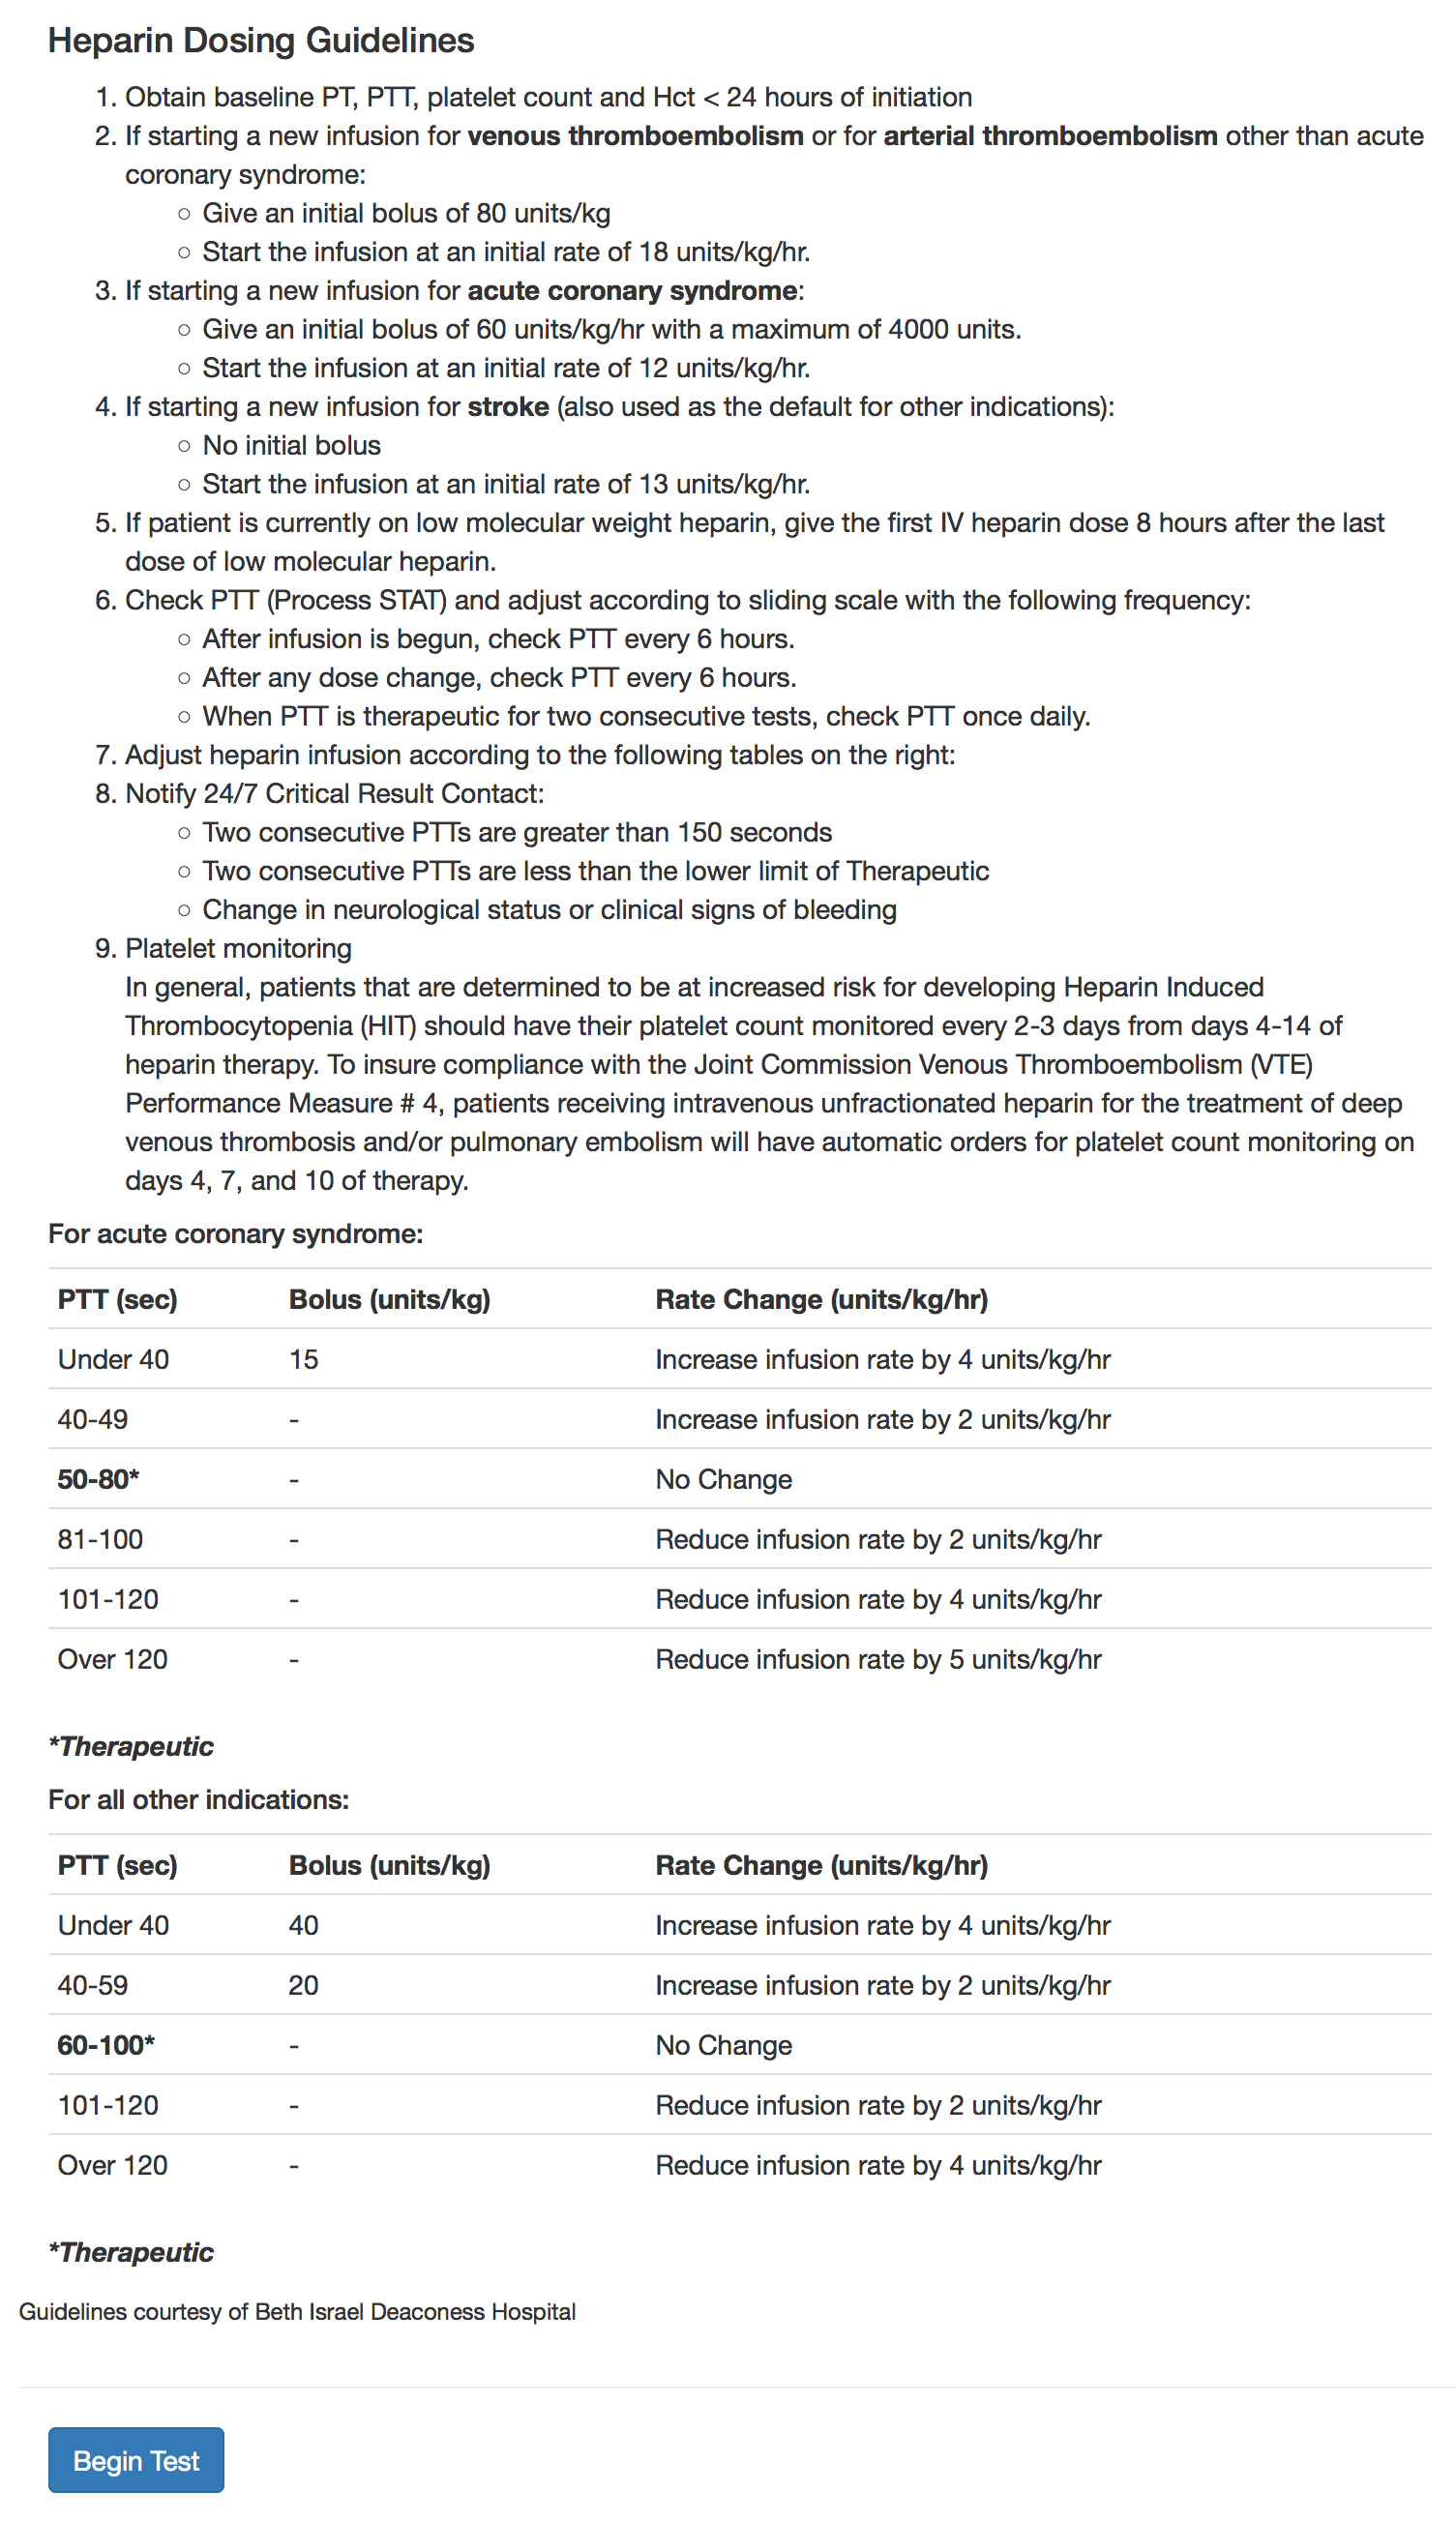
\includegraphics[width=0.8\textwidth]{source/figures/part3info_ii.png}
\caption{\label{fig:part3info2}The standard heparin dosing guidelines participants used throughout the study. The guidelines were always accessible when a participant was asked to prescribe heparin.}
\end{figure}

\begin{figure}[H]
\noindent
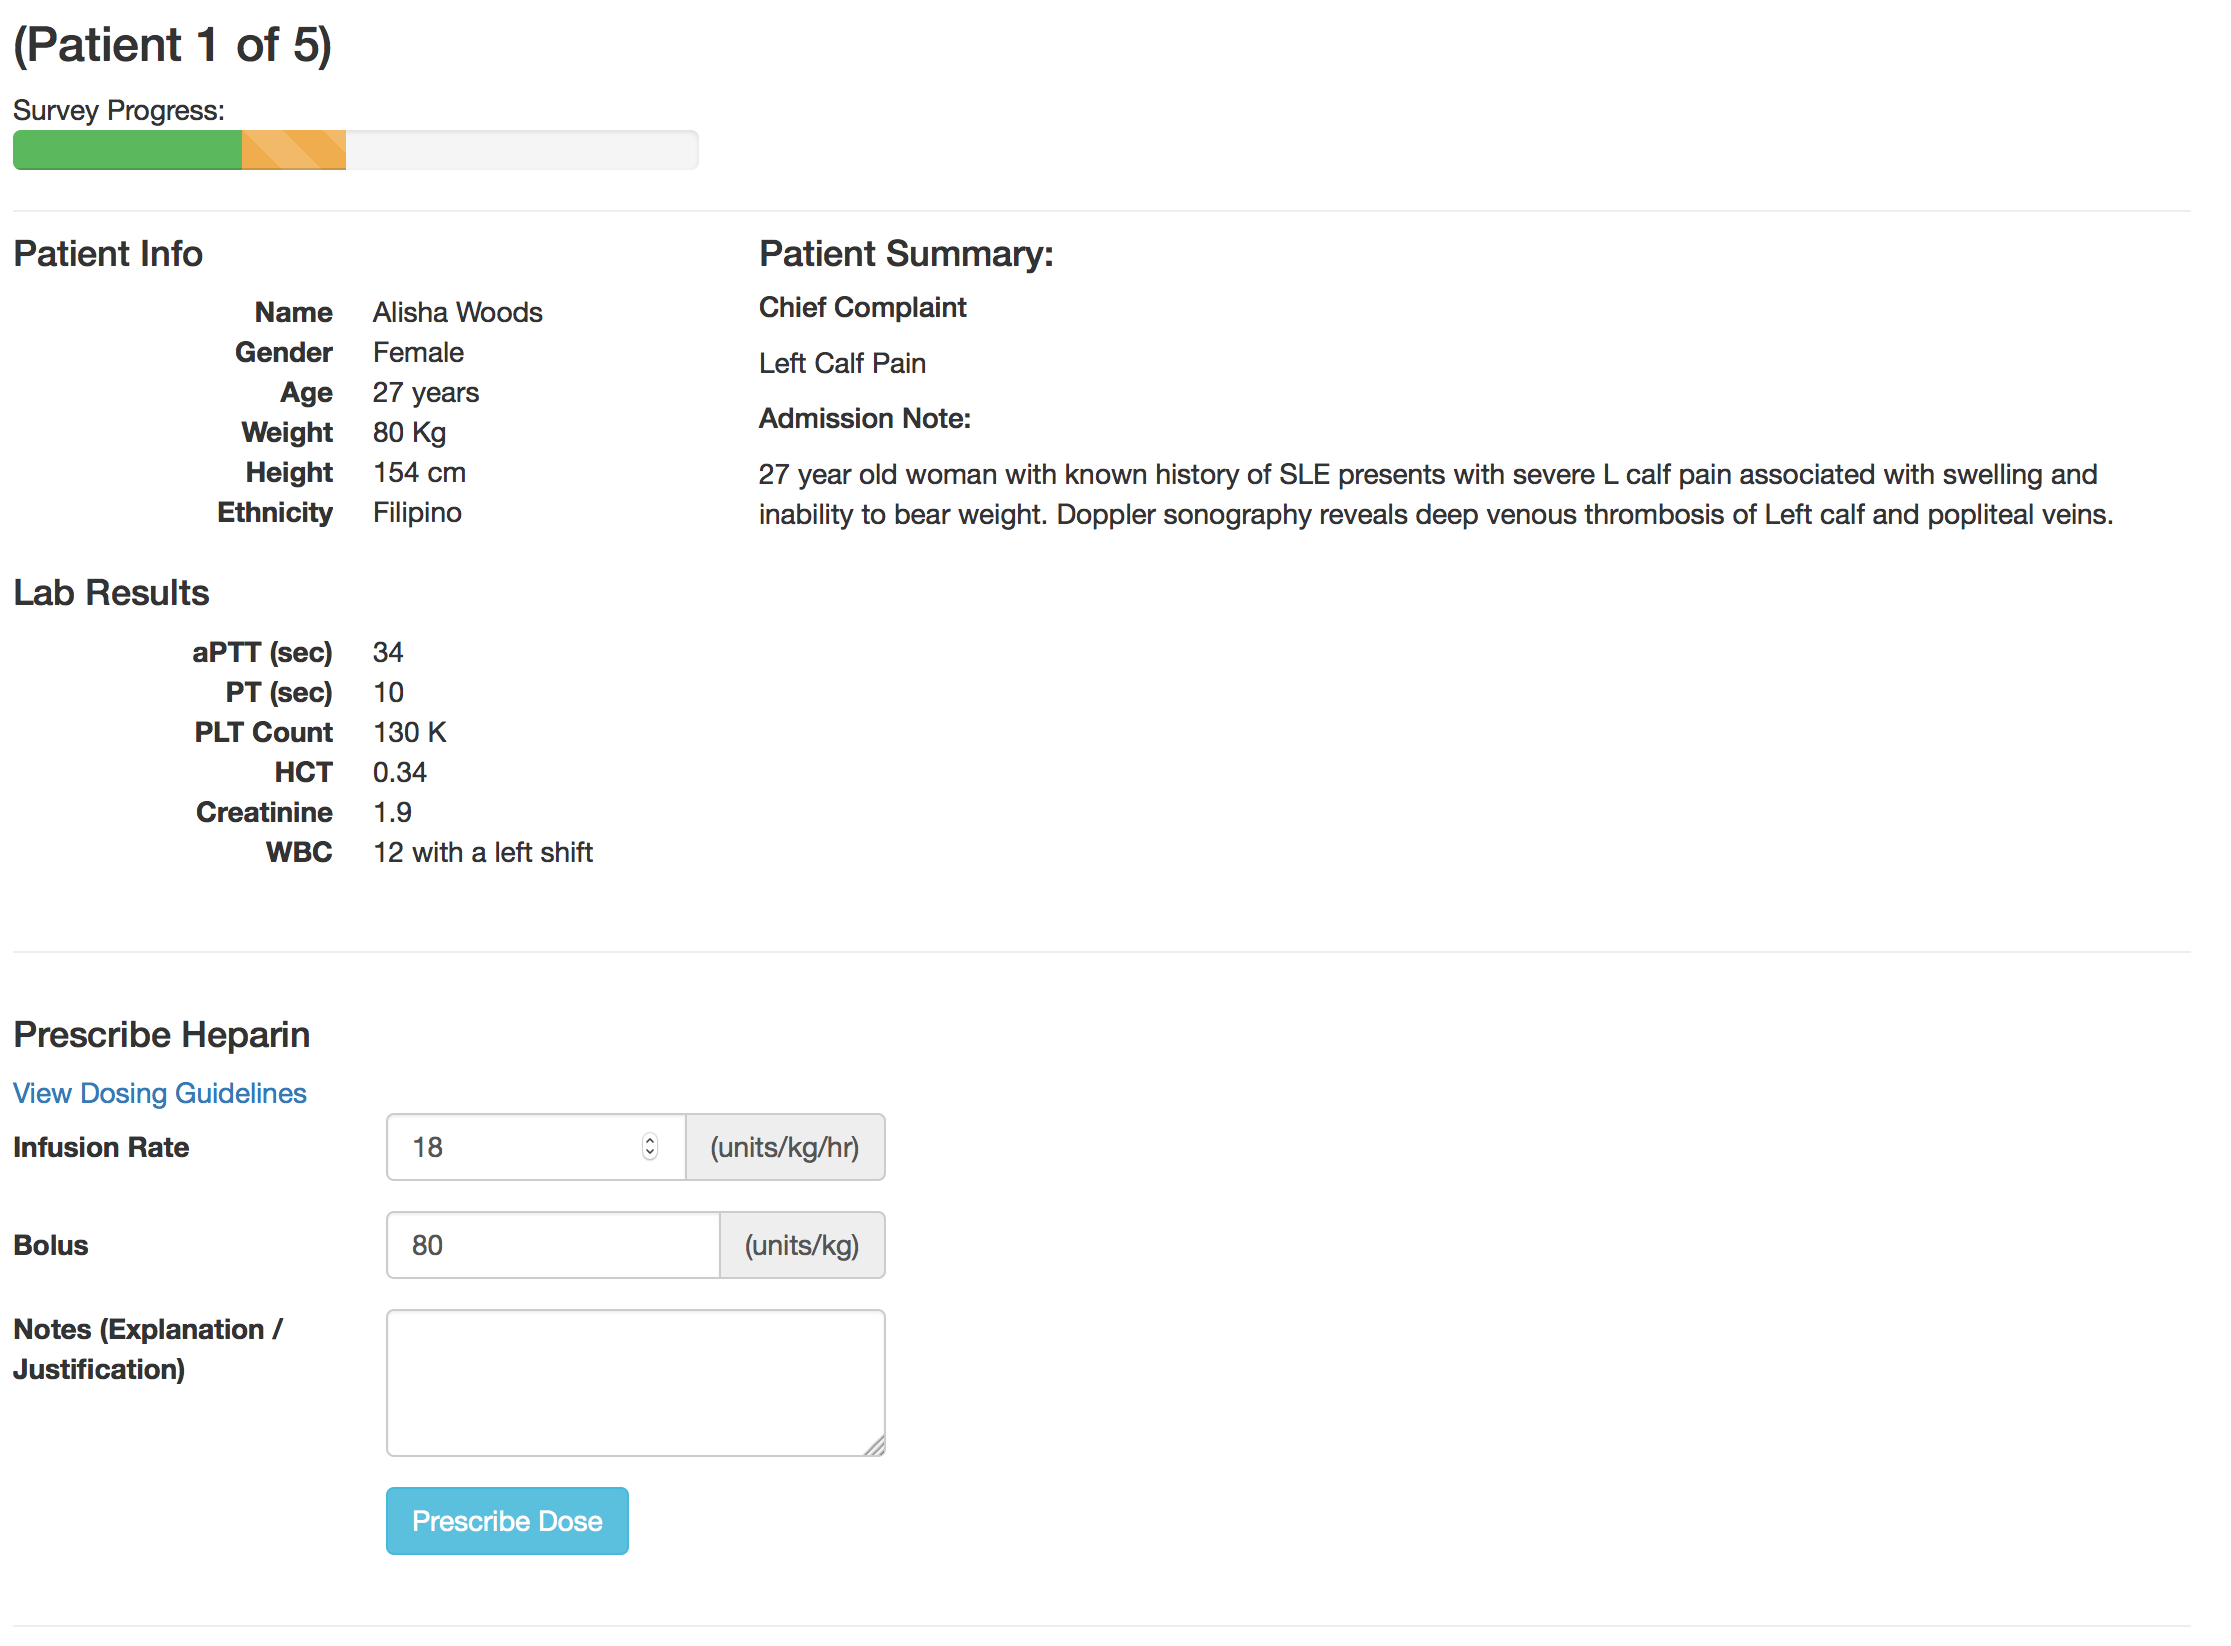
\includegraphics[width=1\textwidth]{source/figures/part3_i.png}
\caption{\label{fig:part3_i}The patient profile and dosing page. In this image the participant has entered in values for the infusion rate and bolus. }
\end{figure}

\begin{figure}[H]
\noindent
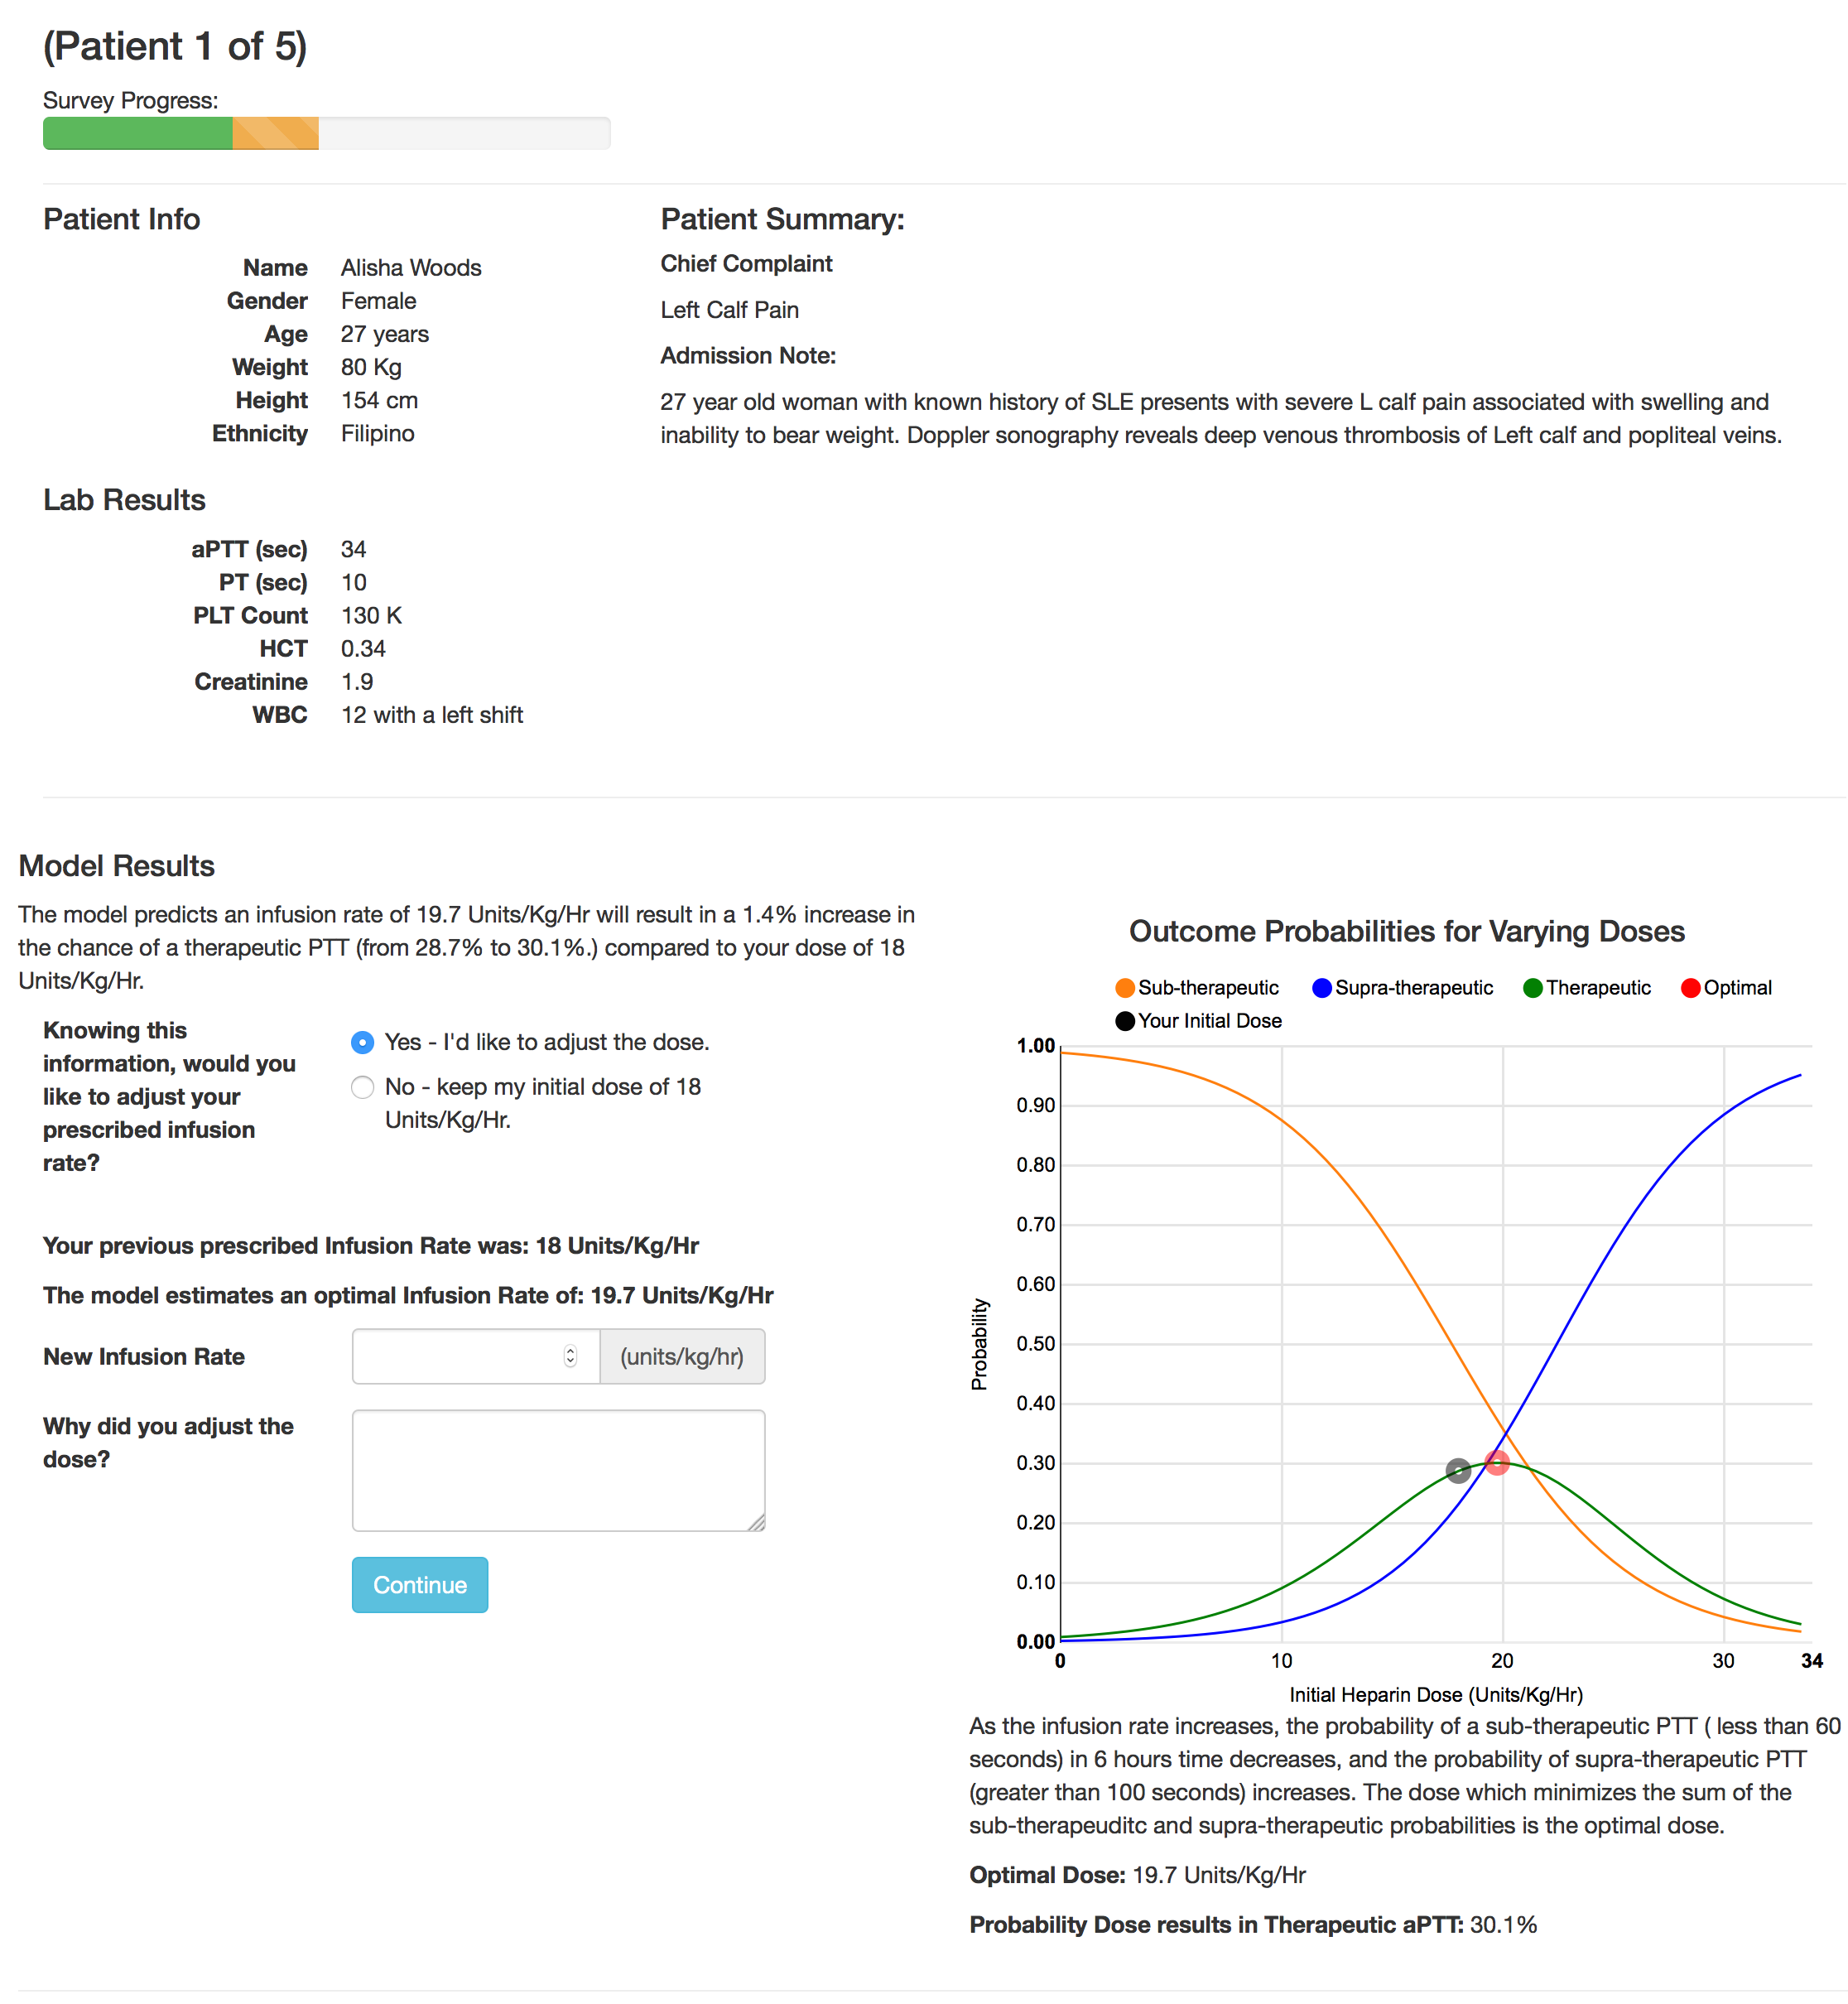
\includegraphics[width=1\textwidth]{source/figures/part3_ii.png}
\caption{\label{fig:part3_ii}The page a study participant sees after selecting an initial infusion rate during the survey. Here the model is displayed and an interface allows them to adjust their initial dose. Note that the system plots the users initial dose (in black) on the therapeutic curve so the user can see how their dose compares to the best estimated dose.}
\end{figure}

\begin{figure}[H]
\noindent
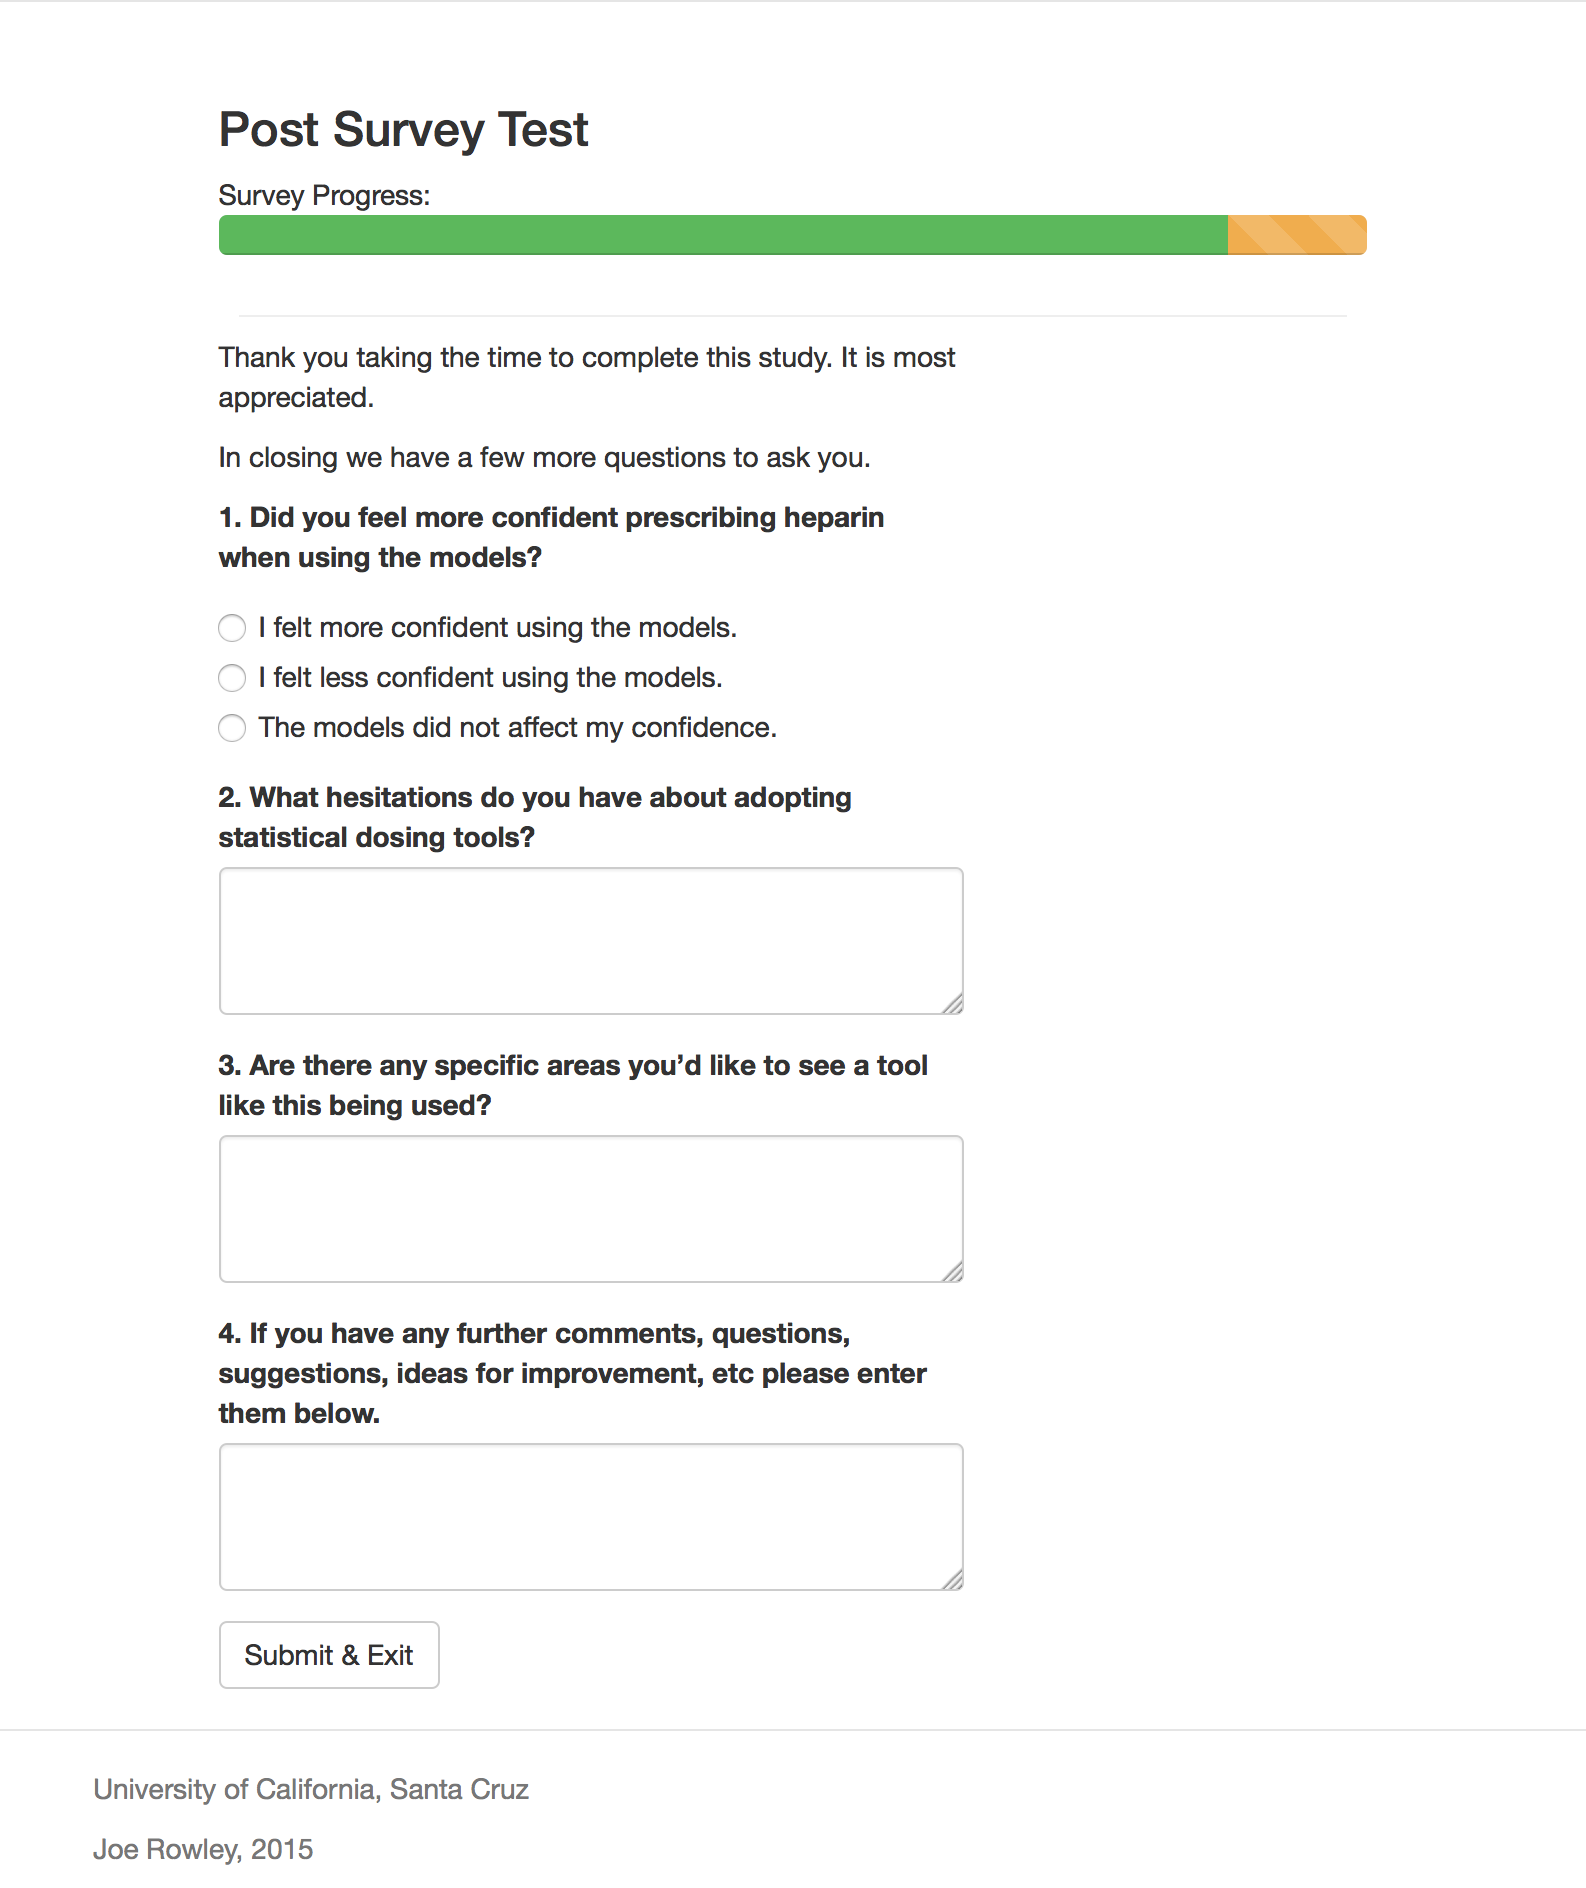
\includegraphics[width=1\textwidth]{source/figures/postsurvey.png}
\caption{\label{fig:postsurvey}The questionnaire presented to study participants after dosing all patients in the previous section.}
\end{figure}

\newpage

\chapter*{Appendix 3: Research
Resources}\label{appendix-3-research-resources}
\addcontentsline{toc}{chapter}{Appendix 3: Research Resources}

Below is an incomplete list of tools I used while creating the
application:

\begin{itemize}
\tightlist
\item
  Web App Tools: Grunt, Bower, NPM
\item
  Typesetting:
  \href{https://github.com/tompollard/phd_thesis_markdown}{Tom Pollard's
  Markdown to Latex Scripts}
\end{itemize}

Below is an incomplete list of tutorials and resources I found helpful
while creating the application:

\begin{itemize}
\tightlist
\item
  Sahil Diwan's
  \href{http://blog.sahildiwan.com/posts/flask-and-postgresql-app-deployed-on-heroku/}{Making
  a Flask app using a PostgreSQL database and deploying to Heroku}
\item
  Yuval Adam's
  \href{http://blog.y3xz.com/blog/2012/08/16/flask-and-postgresql-on-heroku}{Flask
  and PostgreSQL on Heroku}
\item
  Real Python's
  \href{https://realpython.com/blog/python/flask-by-example-integrating-flask-and-angularjs/}{Flask
  by Example - Integrating Flask and AngularJS}
\item
  \href{https://mimic.physionet.org/about/mimic/}{MIMIC-III Critical
  Care Database Documentation}
\item
  Randy Olson's
  \href{https://github.com/rhiever/Data-Analysis-and-Machine-Learning-Projects}{data
  analysis and machine learning projects}
\end{itemize}

Additionally, Google, StackOverflow and the Angular.js documentation
were incredibly helpful.

\newpage

\chapter*{References}\label{references}
\addcontentsline{toc}{chapter}{References}

\hypertarget{refs}{}
\hypertarget{ref-ferri2003volume}{}
Ferri, C., Hernández-Orallo, J. \& Salido, M.A., 2003. Volume under the
rOC surface for multi-class problems. In \emph{Machine learning: ECML
2003}. Springer, pp. 108--120.

\hypertarget{ref-ghassemi2014data}{}
Ghassemi, M.M. et al., 2014. A data-driven approach to optimized
medication dosing: A focus on heparin. \emph{Intensive care medicine},
40(9), pp.1332--1339.

\hypertarget{ref-UWHEP}{}
Lisa Gryttenholm, et a., Dan Hendrickson, 2004. Guidelines for the
therapeutic dosing of heparin. Available at:
\url{http://www.uwhealth.org/files/uwhealth/docs/pdf2/Heparin_Infusion_Guideline.pdf}.

\hypertarget{ref-phd2014}{}
Reka G Szigeti, P., MD, 2014. Anti-xa assay. Available at:
\url{http://emedicine.medscape.com/article/2085000-overview}.

\hypertarget{ref-MIMICII}{}
Saeed, M. et al., 2011. Multiparameter intelligent monitoring in
intensive care iI (mimic-ii): A public-access intensive care unit
database. \emph{Critical Care Medicine}, 39, pp.952--960.

\hypertarget{ref-universityofwashingtonpharmacyservices2014}{}
Washington Pharmacy Services, U. of, 2014. Heparin infusion guidelines.
Available at:
\url{https://depts.washington.edu/anticoag/home/content/heparin-infusion-guidelines}.

\end{document}
